\documentclass{../grid-link-report}
\usepackage{graphicx} % for \resizebox
\usepackage{float}
\usepackage{multirow}
\usepackage{makecell}

\SetClassAssetsDir{../class-assets}
\newcommand{\projectassetsdir}{../project-assets}
\newcommand{\analysisdir}{report-assets/analysis}
\project{Heywood BESS}
\client{Atmos}
\title{Connection Study Report}
\docnumber{HEYWOODBESS-GR-RPT-004}
\issueddate{25 July 2025}
\revision{1-0-0}
\revisionhistorycsvpath{report-assets/revisionhistory.csv}
\clientlogopath{\projectassetsdir/client-logo.jpg}

\colorlet{Line}{red}
\colorlet{Intermediate}{yellow}
\colorlet{Low}{green}




\begin{document}
	% Draft commands
	%\adddraftstamp
	
	\frontmatter
	\maketitle
	
	\makedisclaimer
	\clearpage
	\tableofcontents
	\makerevisionhistorypage
%	\makeaboutgridlink
	
	\mainmatter
	

	\chapter{Purpose}
	This document has been prepared as part of the application for Registration for \ac{Heywood BESS}. It presents a technical assessment of the compliance of the generating system to its agreed \ac{GPS} for \ac{GPS} clauses that have been assessed as part of the Connection Studies undertaken at R0 stage, such as fault performance. Table \ref{tab:access-standard-summary} provides a summary of the NER clauses assessed and identifies which clauses are examined in this report\footnote{Note that for some clauses, only the subclauses relevant to dynamic studies are addressed in this report, such as the rapid active power reduction for over-frequency events required by s5.2.5.8}.
	
	% Access standards summary table
	{%
		\thicktablelines
		\begin{longtable}{|>{\columncolor{gray!20}}C{3cm}|C{5cm}|C{2cm}|C{2cm}|C{2cm}|} 
			\caption{Summary of access standards}
			\label{tab:access-standard-summary}
			\\	
			\toprule
			
			\rowcolor{tableheaderblue}
			\bfseries \bfseries \color{white}Clause & \bfseries \color{white}Description & \bfseries \color{white}Version & \bfseries \color{white}Standard & \bfseries \color{white}In Scope \\
			\endhead
			\bottomrule \endfoot
			\csvreader[
			separator=comma,
			late after line=\\\hline,
			late after last line=,
			before reading={\catcode`\#=12},
			after reading={\catcode`\#=6}]%
			{\projectassetsdir/access_standards_summary.csv}{1=\CSVClause,2=\CSVDescription,3=\CSVVersion,4=\CSVStandard,5=\CSVInScope}{\CSVClause & \CSVDescription & \CSVVersion & \CSVStandard & \CSVInScope}
			
		\end{longtable}
	}
	
	\chapter{Project Overview}
	
	The Heywood Battery Energy Storage System (HEYWOODBESS) is a $\pm~285MW/1140MWh$ Battery Energy Storage Project, is located 5 km from the town of Heywood and 300 km west of Melbourne in Victoria as shown in Figure~\ref{fig:project-location}. The project is expected to connect directly to the existing 275 kV Heywood terminal station via a single high voltage cable.

HEYWOODBESS will include 92 SMA Sunny Central 4.6 MVA (SCS 4600 UP-S) converters which will be connected to two 275/33/33kV, 160MVA three winding transformers through a 33kV reticulation system. Each converter will have a dedicated 33/0.69kV, 4.6 MVA step up transformer.


\begin{figure}[H]
	\centering
	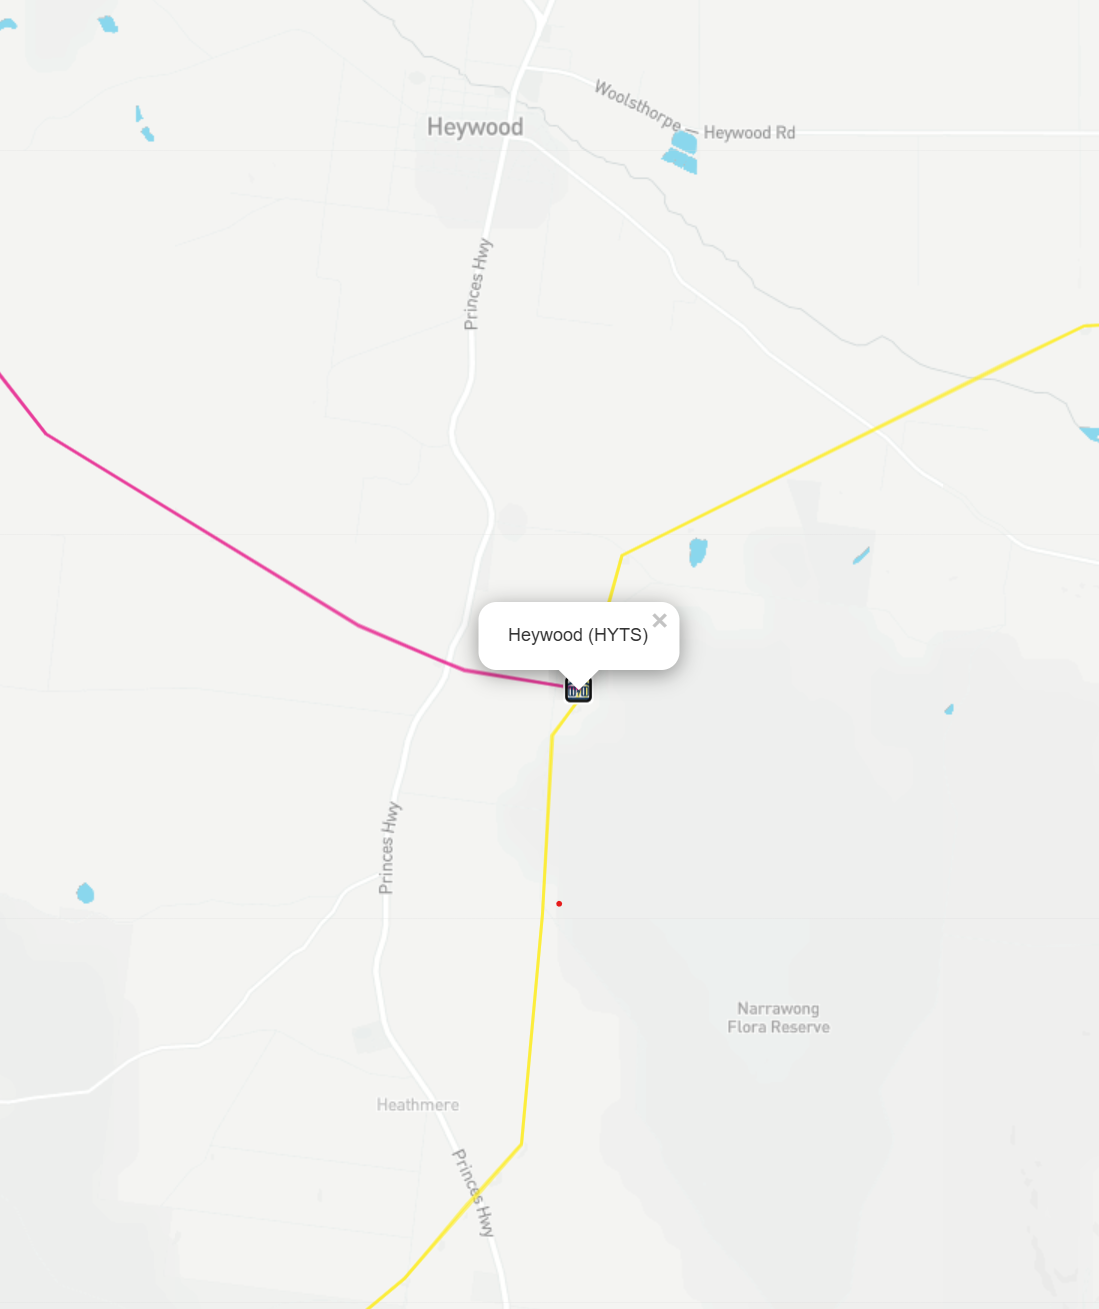
\includegraphics[width=0.7\textwidth]{\projectassetsdir/project-location.png} % Change example-image-a to the filename of your image
	\caption{Project location}
	\label{fig:project-location}
\end{figure}


	
	\chapter{Performance Standards}
	\section{[S5.2.5.1] Reactive Power Capability}
	\subsection{Proposed Access Standard}
	\textbf{Automatic Access Standard}
	\begin{tcolorbox}[lightgreenbox]
		Integrated resource system's rated active power = 285 MW as measured at the Connection Point.

While operating at any level of active power output and at any voltage at the Connection Point within the limits of ±10\% of Normal Voltage, the integrated resource system is capable of supplying and absorbing at the Connection Point an amount of reactive power at least equal to the product of the rated active power of the integrated resource system and 0.395, as reflected in Figure 1.

\begin{figure}[H]
	\centering
	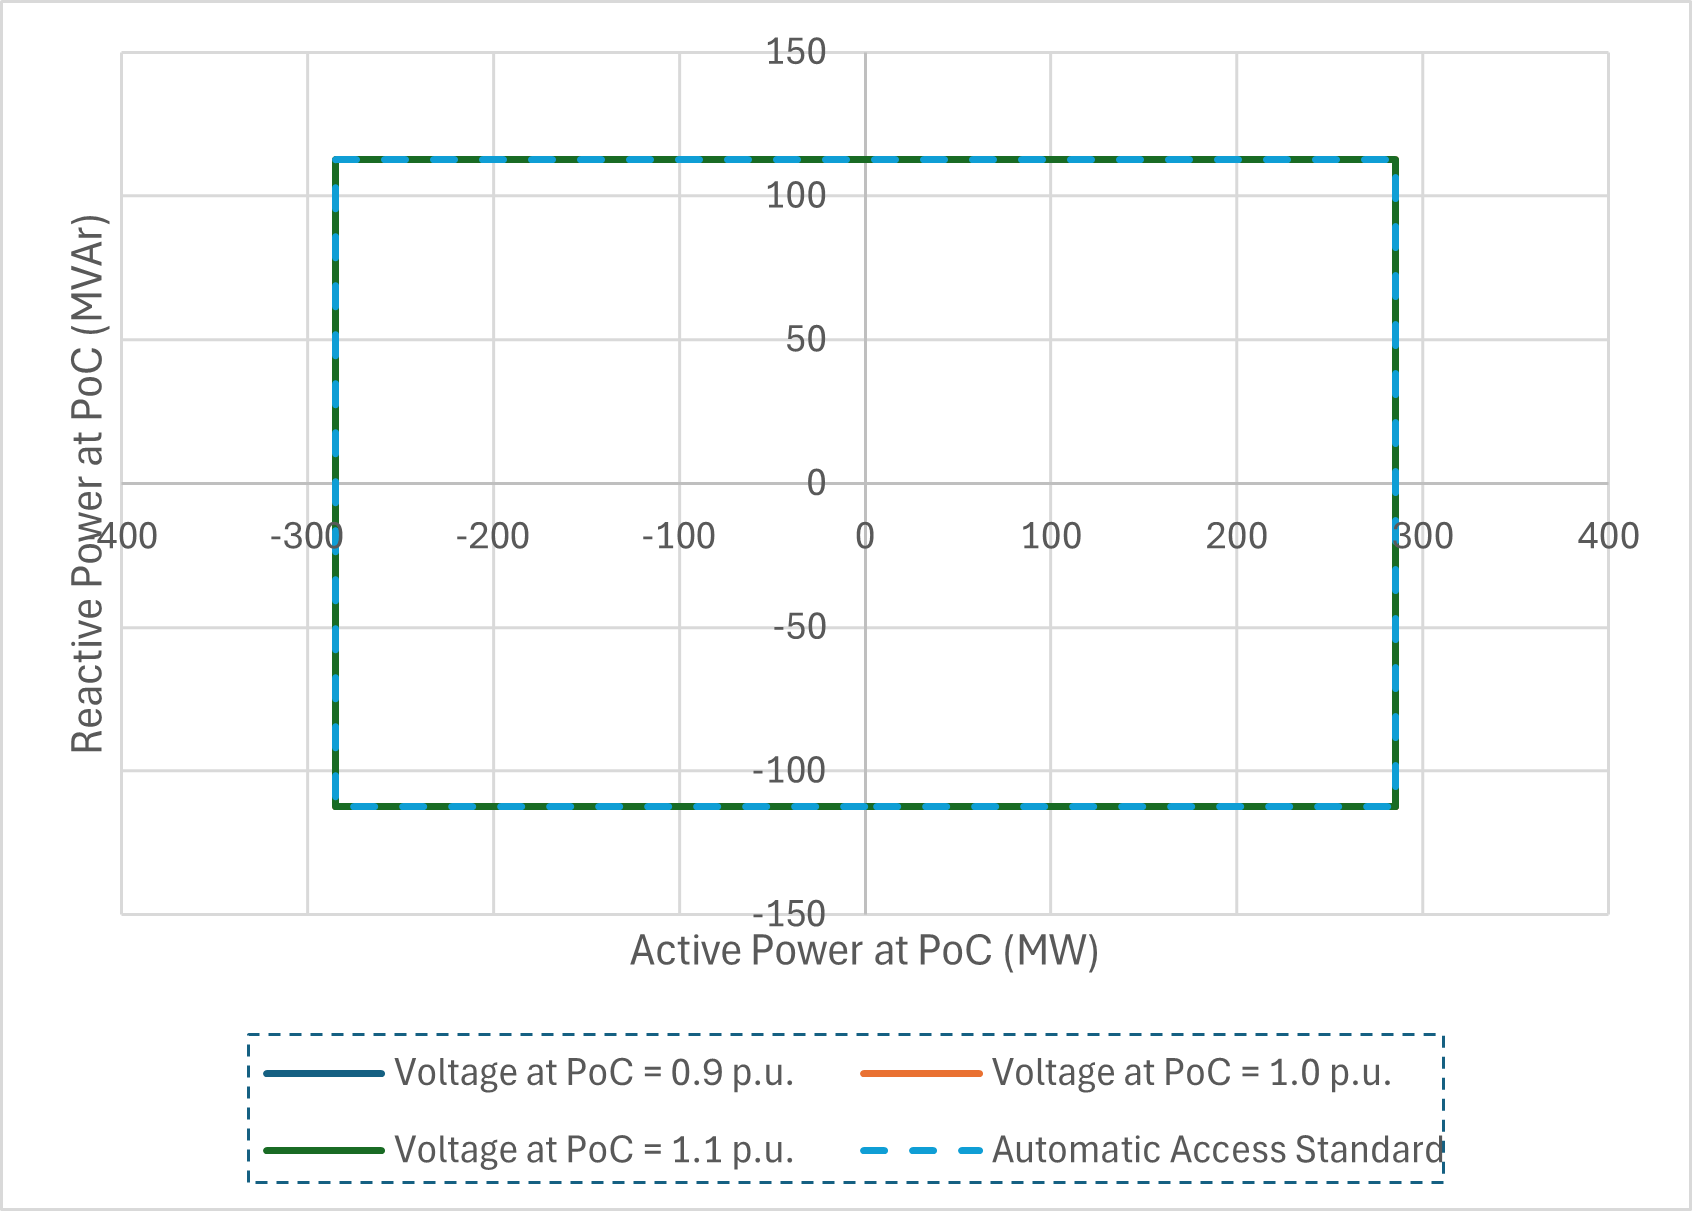
\includegraphics[width=0.8\textwidth]{\projectassetsdir/gps-clauses/s5251-curve.png}
\end{figure}
\textbf{Figure 1: Reactive power capability up to 50°C rating}

The integrated resource system, while not generating active power and not supplying or absorbing reactive power under an ancillary services agreement:
\begin{itemize}
	\item When the production units are connected and the ambient temperature is less than 50OC, follow the voltage regulation control requirement specified in the performance standard under clause S5.2.5.13 with a reactive power capability of ± 1.223 MVAr for each production unit; and
	\item When the production units are not connected, not supply at its Connection Point reactive power of more than 0 MVAr and not draw more electricity than XXXX kW of active power and XXXX kVAr of reactive power;
\end{itemize}

If the reactive power supplied or absorbed at the Connection Point falls outside the range that applies when the production units are not connected, the integrated resource system must, where required by the NSP in order to maintain satisfactory voltage levels at the Connection Point or to restore intra-regional or inter-regional power transfer capability, take action to ensure that the reactive power falls within that range within 30 min.

	\end{tcolorbox}
	
	
	\subsection{Assessment Methodology}
	Reactive capability studies have been performed on a full, detailed model of the plant (including all cables, inverters and transformers), based on inverter reactive capability curves supplied by the OEM. Powerfactory is capable of interpolating between these curves, allowing for accurate reactive power output to be calculated based on the individual terminal voltages of each inverter\footnote{Note that Powerfactory is not capable of doing the same for active power, so invalid active power values are removed in post-processing.}. 

For each ambient temperature and connection point voltage to be studied, the appropriate capability curve for the inverter is applied and the connection point voltage is fixed to the target level. With the transformers permitted to tap, the case is first solved with all inverters exporting as much reactive power as possible without leaving their range of terminal voltages for which they are able to individually maintain \ac{CUO}. This study is repeated with all inverters importing as much reactive power as possible while maintaining \ac{CUO}. Both processes are then repeated for all levels of inverter active power dispatch and a complete reactive capability curve is developed by recording the connection point active and reactive power outputs for all studies.

To confirm \ac{CUO} is maintained at a generating system level for s5.2.5.4, the same study is repeated, but prior to recording the results, the transformer \acp{OLTC} are locked, and the connection point voltage is stepped to the extents of the \ac{CUO} voltage band or $\pm10\%$, whichever is less onerous\footnote{Per AEMO recommended rule change}. The results for these studies are recorded as alternative, more onerous "\ac{CUO} curves."

The remainder of the s5.2.5.1 clause consists of restrictions around the following:

\begin{enumerate}
	\item How much active and reactive power can be imported or exported by the generating system when the inverters are connected but not generating active power, which allows for the consideration of the inverters' reactive power at night feature, but does not allow for the filters to be out of service as they are required to offset the harmonics produced by inverters in this mode. In the operations phase, this would be a time when the generator has bid out, is curtailed or has no available power (e.g. due to it being night time).
	\item When the inverters are disconnected, which allows for the disconnection of the harmonic filter and even the 33kV circuit breaker, as this would only occur if there was a significant problem with the control system or a planned maintenance outage of the whole generating system.
\end{enumerate} 

Assessment for this clause has been performed using PowerFactory.
	
	One change to the standard methodology was allowed for this plant. The plant is equipped with an OLTC which can operate within the normal voltage ride through capability of the Sungrow converters used on this project, which can operate for terminal voltages well outside those that would occur under normal operation at the POC of 0.9 to 1.1 p.u. voltage. The ride through capability of these converters is shown in the Sungrow datasheet \cite{sungrow-lvrt-and-hvrt}, permits operation at voltages of up to 1.2 p.u or down to 0.5 p.u. at the converter terminals for up to 60 seconds.
	
	This expanded range of operation was reflected by allowing the project OLTC to perform a tapping action twice under continuous uninterrupted operation testing. This action reflected the plant capability to reduce or increase terminal voltage and allowed an expanded range of reactive capability. Two tapping actions within 60 seconds are permitted by the design of the OLTC, which is set to a 20 second delay for operation, and will require 7 seconds to mechanically operate.
	
	\subsection{Results}
	
	The reactive capability curves for HEYWOODBESS at 35°C, 45°C and 50°C are shown in Figures \ref{fig:pq-curve-35degC}, \ref{fig:pq-curve-40degC} and \ref{fig:pq-curve-50degC}. Detailed results in .xslx format can be found in the Capability Curves folder of the R0 submission.
	
	\begin{figure}[H]
		\centering
		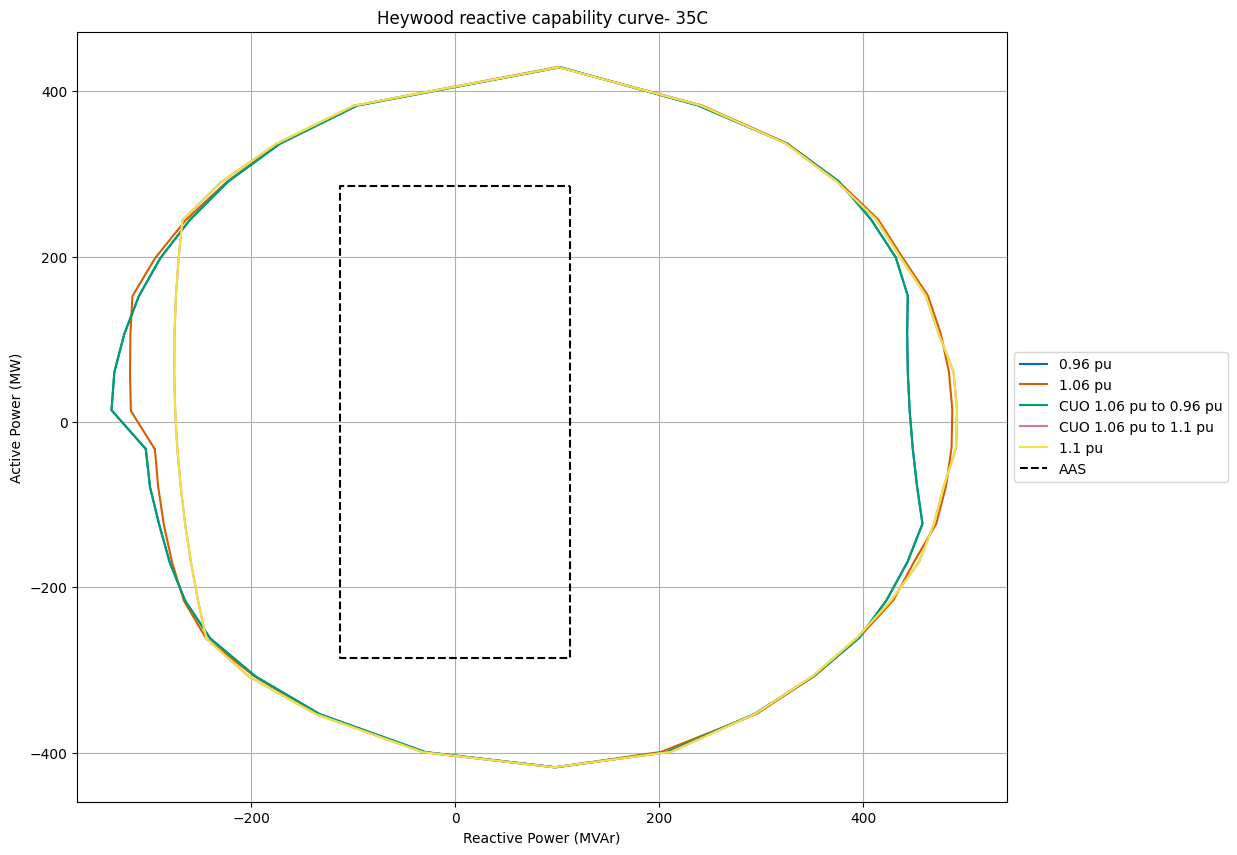
\includegraphics[width=0.8\textwidth]{\projectassetsdir/capability-curves/new_Heywood reactive capability curve- 35C.png}
		\caption{35°C Reactive capability curve for HEYWOODBESS}
		\label{fig:pq-curve-35degC}
	\end{figure}
	
	\begin{figure}[H]
		\centering
		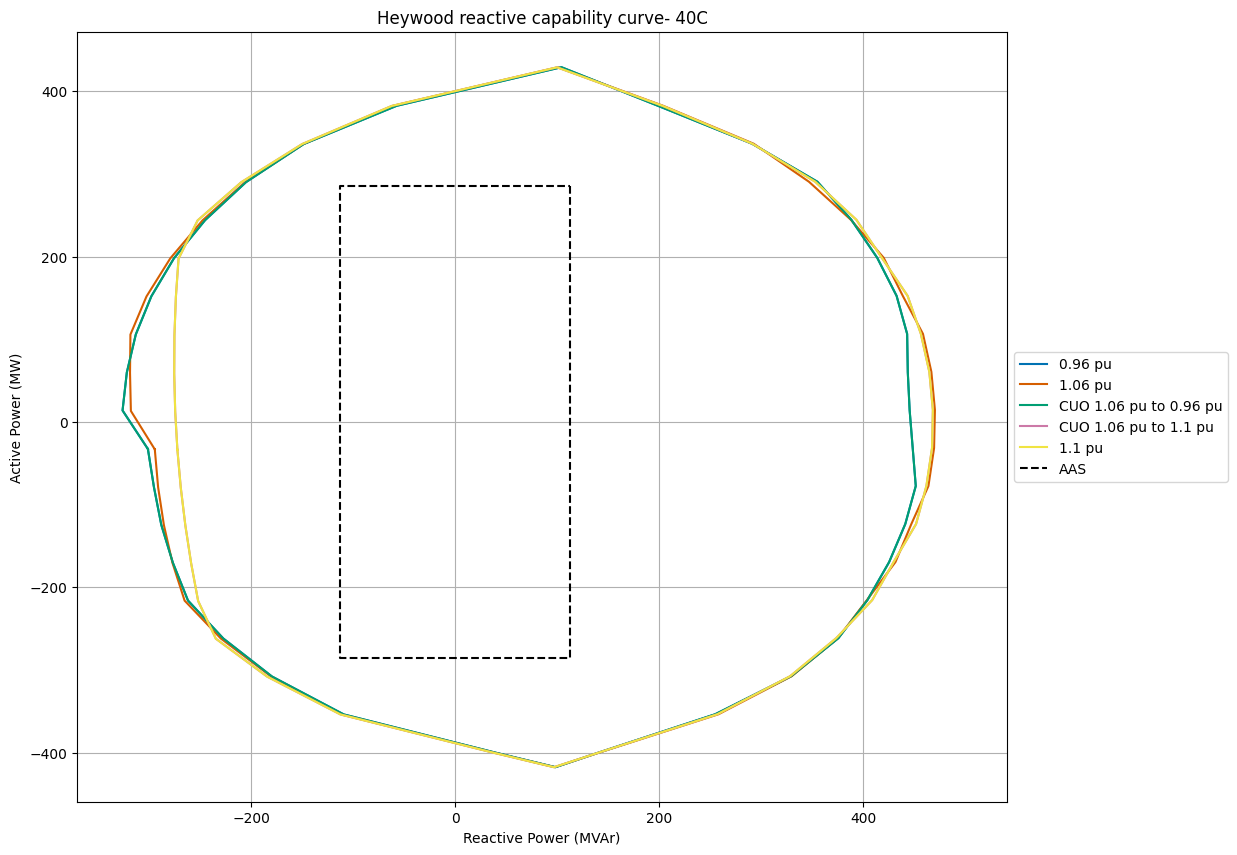
\includegraphics[width=0.8\textwidth]{\projectassetsdir/capability-curves/new_Heywood reactive capability curve- 40C.png}
		\caption{40°C Reactive capability curve for HEYWOODBESS}
		\label{fig:pq-curve-40degC}
	\end{figure}
	
	\begin{figure}[H]
		\centering
		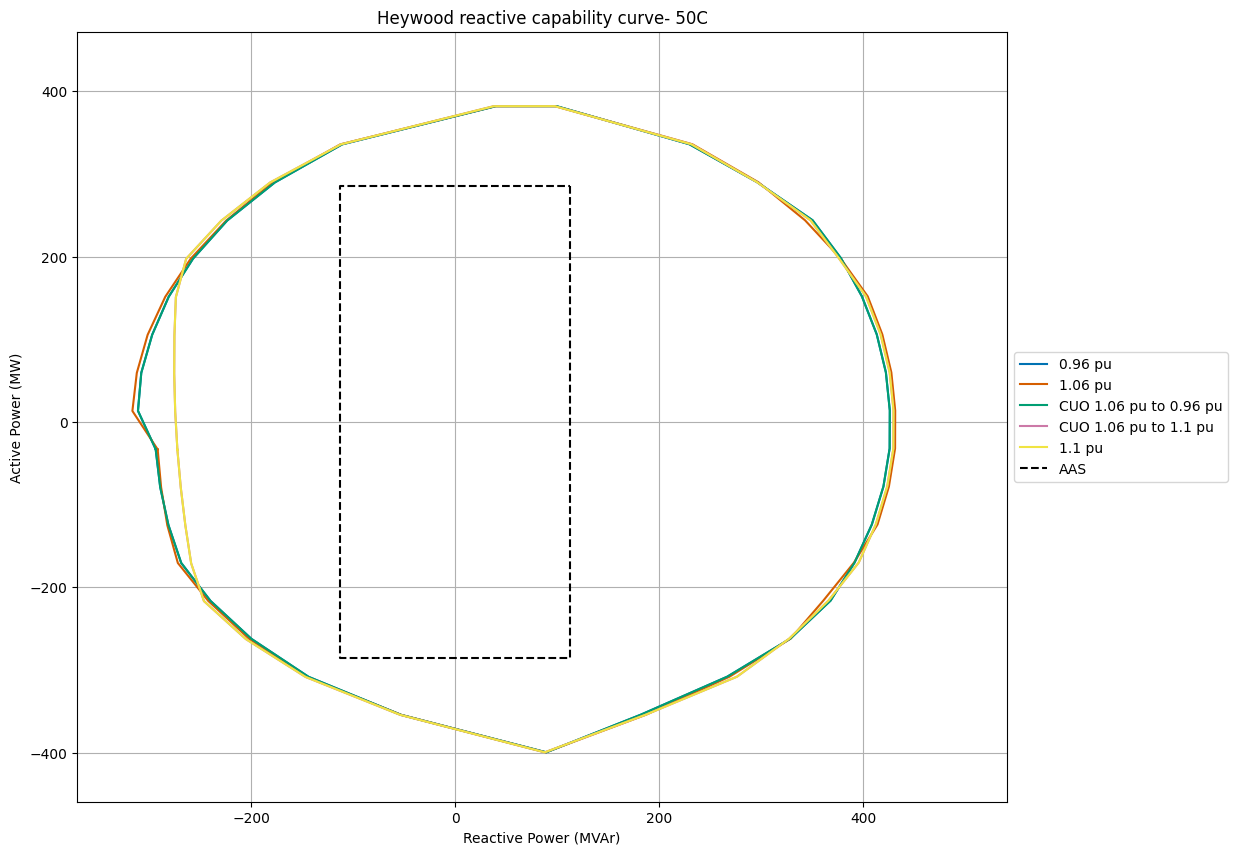
\includegraphics[width=0.8\textwidth]{\projectassetsdir/capability-curves/Heywood reactive capability curve- 50C.png}
		\caption{50°C Reactive capability curve for HEYWOODBESS}
		\label{fig:pq-curve-50degC}
	\end{figure}
	
	Table \ref{tab:s5251-power-draw-when-inverters-disconnected} shows the that the amount of active power and reactive power consumption from the generator when all generating units are disconnected, and harmonic filters are switched out of service is minor. However, it is noted that the DIgSILENT model only accounts for the power drawn by the reticulation network and converter transformers, and not for auxiliary loads.  The performance standard proposed for the BESS therefore is set in excess of these figures at 3500 kW and 2000 kVAr, which have been set to reflect additional auxiliary loads such as the requirements for heating, cooling and lighting at the facility, which will be confirmed during detailed design.

	\begin{table}[H]
		\centering
		\begin{tabular}{|c|c|c|c|c|}
			\hline
			$V_{\mathrm{POC}}$ & Filters & 33kV Reticulation & $P_{\mathrm{POC}}$ & $Q_{\mathrm{POC}}$  \\ \hline
			0.9 pu & Out Of Service & In Service & 0.415 MW & -0.092 MVAr \\ \hline
			1.1 pu & Out Of Service & In Service & 0.620 MW & -0.138 MVAr \\ \hline
		\end{tabular}
		\caption{Active and reactive power import/export when inverters are disconnected.}
		\label{tab:s5251-power-draw-when-inverters-disconnected}
	\end{table}

	\section{[S5.2.5.2] Quality of Electricity Generated}
	\subsection{Proposed Access Standard}
	\textbf{Negotiated Access Standard}
		\begin{tcolorbox}[lightgreenbox]
			%\documentclass{article}
%\usepackage{graphicx}
%\begin{document}
	
	\begin{itemize}
		\item When generating and when not generating, the integrated resource system does not produce at the Connection Point:
		\begin{itemize}
			\item[(a)] Voltage fluctuations greater than the limits specified in Table 2.1 by the NSP under clause S5.1.5(a) of the NER, where flicker will be measured in accordance with AS/NZS 61000.3.7:2001:
		\end{itemize}
		
			\begin{center}
			\begin{tabular}{|c|c|}
				\hline
				\textbf{Pst} & \textbf{Plt} \\
				\hline
				0.35 & 0.25 \\
				\hline
			\end{tabular}
			\end{center}
		
		\begin{itemize}
			\item[(b)] Harmonic voltage distortion greater than the limits specified in Table 2.2 by the NSP under clause S5.1.6(a) of the NER and will be measured at the Connection Point in accordance with AS/NZS 61000.3.6:2001:
		\end{itemize}
		
			\begin{center}
			\begin{tabular}{|p{2cm}|p{2cm}|p{2cm}|p{2cm}|p{2cm}|p{2cm}|}
				\hline
				\textbf{Harmonic Order (h)} & \textbf{Harmonic Voltage Limits (\%)} & \textbf{Harmonic Order (h)} & \textbf{Harmonic Voltage Limits (\%)} & \textbf{Harmonic Order (h)} & \textbf{Harmonic Voltage Limits (\%)} \\
				\hline
				2 & 0.1 & 19 & 0.12 & 36 & 0.1 \\
				3 & 0.1 & 20 & 0.1 & 37 & 0.1 \\
				4 & 0.1 & 21 & 0.1 & 38 & 0.1 \\
				5 & 0.1 & 22 & 0.1 & 39 & 0.1 \\
				6 & 0.1 & 23 & 0.1 & 40 & 0.1 \\
				7 & 0.1 & 24 & 0.1 & 41 & 0.1 \\
				8 & 0.1 & 25 & 0.1 & 42 & 0.1 \\
				9 & 0.1 & 26 & 0.1 & 43 & 0.1 \\
				10 & 0.1 & 27 & 0.1 & 44 & 0.1 \\
				11 & 0.18 & 28 & 0.1 & 45 & 0.1 \\
				12 & 0.1 & 29 & 0.1 & 46 & 0.1 \\
				13 & 0.18 & 30 & 0.1 & 47 & 0.1 \\
				14 & 0.1 & 31 & 0.1 & 48 & 0.1 \\
				15 & 0.1 & 32 & 0.1 & 49 & 0.1 \\
				16 & 0.1 & 33 & 0.1 & 50 & 0.1 \\
				17 & 0.12 & 34 & 0.1 & THD & 0.23 \\
				18 & 0.1 & 35 & 0.1 & & \\
				\hline
			\end{tabular}
			\end{center}
		
		\begin{itemize}
			\item[(c)] Voltage unbalance greater than the limits specified in Table 2.3 by the NSP under clause S5.1.7(c) of the NER and will be measured in accordance with AS/NZS 61000.3.6:2001:
		\end{itemize}
		
			\begin{center}
			\begin{tabular}{|p{3cm}|p{2cm}|p{2cm}|p{2cm}|p{2cm}|}
				\hline
				\multirow{2}{*}{{\makecell{\textbf{Nominal Supply} \\ \textbf{Voltage (kV)}}}} & \multicolumn{4}{c|}{\textbf{Maximum Negative Sequence Voltage (\% of Nominal Voltage)}} \\ 
				\cline{2-5}
				& \textit{No contingency event} (30-min average) & \textit{Credible contingency event} (30-min average) & General (10-min average) & Once per hour (1-min average) \\ 
				\hline
				275 & 0.5 & 0.7 & 1.0 & 2.0 \\ 
				\hline
			\end{tabular}
			\end{center}
	\end{itemize}
	
%\end{document}

		\end{tcolorbox}
	
	\subsection{Assessment Methodology}
		Detailed assessment of the ability of the integrated resource system to meet this performance standard has been undertaken in a separate power quality report. \cite{power-quality-report}

	\section{[S5.2.5.3] Generating System Response to Frequency Disturbances}
		\subsection{Proposed Access Standard}
		\textbf{Automatic Access Standard}
			\begin{tcolorbox}[lightgreenbox]
					Unless the rate of change of frequency is outside the range of ±4 Hz/s for more than 0.25 s, ±3 Hz/s for more than 1.00 s, the integrated resource system and each of its production units is capable of continuous uninterrupted operation for frequencies in the ranges indicated in Table 2.4:
	

	\begin{table}[H]
		\centering
		\begin{tabular}{|c|c|}
			\hline
			\textbf{Frequency Range (Hz)\textsuperscript{(1)}} & \textbf{Duration\textsuperscript{(1)}} \\ \hline
			47 to 48 & 2 min \\ \hline			
			48 to 49.5 & 10 min \\ \hline			
			49.5 to 50.5 & continuous \\ \hline
			50.5 to 52 & 10 min \\ \hline
		\end{tabular}
		\caption*{Table 2.4:  Frequency Limits for Continuous Uninterrupted Operation}
	\end{table}
	Notes:  
	
	\textsuperscript{(1)} Based on the frequency operating standard effective 1 January 2020.
	

	
			\end{tcolorbox}
			
		\subsection{Assessment Methodology}
			To assess this clause, a series of 'envelope' tests were performed, where the system frequency was initialised at 50Hz, then ramped to the furthest extent of the \ac{OFRT} or \ac{UFRT} ride-through bands, then gradually ramped down such that each band is sustained for the required duration. The results are then analysed to confirm that no generating units tripped during the study.

To implement these tests, $F_{\mathrm{grid}}$ is driven with a time-series signal $F_{\mathrm{grid}_{\mathrm{1}}}, F_{\mathrm{grid}_{\mathrm{2}}}, F_{\mathrm{grid}_{\mathrm{3}}}, \dots, F_{\mathrm{grid}_{\mathrm{n}}}$, as shown in Figure~\ref{fig:s5253-assessment-methodology}. The assessment is performed on an infinite grid.

\begin{figure}[H]
	\centering
	
	\newcommand{\bushere}[3]{% length, text above, text below}
	% Optional arguments do nto work in paths
	%
	% starting point; draw an edge and then two nodes
	% save the position
	coordinate(tmp)
	% go up and do an edge down
	++(0,#1) node[anchor=base, font=\footnotesize]{#2} edge[ultra thick] ++(0, {-2*#1})
	% edges do not move the current point, go down to position the node
	++(0,{-2*#1}) node[below]{#3}
	% go back to where we started
	(tmp)
	}
	
	\ctikzset{sources/fill=gray!20, resistors/fill=gray!20}
	\resizebox{0.7\linewidth}{!}{ % Set width to \linewidth
	\begin{tikzpicture}[semithick]% default line width
		% Buses and branches
		\draw (0,0)
		node[left, font=\footnotesize]{Generator} ++(1.5,0) \bushere{1.5}{Connection Point}{} coordinate(poc);
		\draw (poc) -- ++(1,0) node[vsourcesinshape, rotate=90]{} coordinate(vgrid) ++(0.5,0) node[right]{$V_{\text{grid}}$};
		\draw (poc) -- ++(-1,0) node[vsourcesinshape, rotate=90]{};
		% Fault
		\draw[blue, font=\footnotesize, <-] (vgrid) ++(0, -0.5) -- ++(0, -0.5) -- ++(0.5,0) node[right]{$F_{\mathrm{grid}_{\mathrm{1}}}, F_{\mathrm{grid}_{\mathrm{2}}}, F_{\mathrm{grid}_{\mathrm{3}}}, \dots, F_{\mathrm{grid}_{\mathrm{n}}}$};
		
	\end{tikzpicture}
	}	
	\caption{s5.2.5.3 assessment methodology}
	\label{fig:s5253-assessment-methodology}
\end{figure}
		
			All assessments for this clause have been performed in PSCAD.
			
		\subsection{Results}
			
			The under-frequency and over-frequency ride through performance of the generating system during the envelope tests (performed in PSCAD) relative to the agreed access standard is shown  in \ref{fig:s5253-pscad-frt}. The project was able to remain connected and in continuous uninterrupted operation for the applied "envelope tests" to simulate the frequency withstand requirements of S5.2.5.3.  A summary of the envelope tests performed to produce this plot are shown in Table \ref{tab:s5253-test-suite}. Plots showing these envelope tests are shown in Appendix \ref{Grid Frequency Disturbance Withstand Tests}.
			
			\begin{figure}[H]
				\centering
				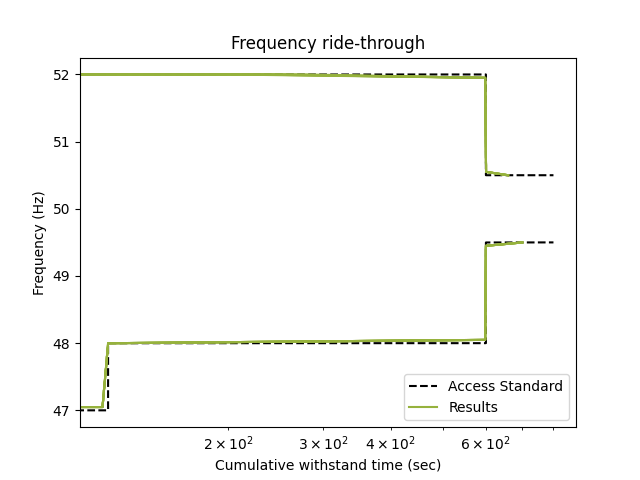
\includegraphics[width=0.7\textwidth]{\analysisdir/pscad/s5253_ride_through_results.png}
				\caption{Frequency ride-through performance}
				\label{fig:s5253-pscad-frt}
			\end{figure}
			
			It should be noted that due to the grid-forming technology inherent to the design of the BESS control systems, the BESS will respond to frequency changes with a virtual "inertial response". While this response is limited by the maximum current supplied by the BESS, the BESS can exceed its maximum active power output rating on a short term basis as a result of this inertial response. This response is inherent to the control strategy of the BESS in grid-forming mode, and is similar in nature to the inertial response of a synchronous generator.
			
			\begin{table}[H]
				\centering
				\caption{s5.2.5.3 frequency ride-through test suite}
				\label{tab:s5253-test-suite}
				\autoscaledtable{H}{\projectassetsdir/test-suite-tables/5253-test-table.csv}
			\end{table}



	\section{[S5.2.5.4] Generating System Response to Voltage Disturbances}
		\subsection{Proposed Access Standard}
		\textbf{Automatic Access Standard}
			\begin{tcolorbox}[lightgreenbox]
				The integrated resource system and each of its production units is capable of continuous uninterrupted operation where a power system disturbance causes the voltage at the Connection Point to vary within the ranges indicated in Table 2.5:

\begin{table}[H]
	\centering
	\resizebox{0.6\textwidth}{!}{%
		\begin{tabular}{|c|c|}
			\hline
			\textbf{Voltage Range (\% of Normal Voltage)} & \textbf{Duration} \\ \hline
			
			>130\% & 0.02 s\textsuperscript{(1)} \\ \hline
			125\% to 130\% & 0.2 s\textsuperscript{(1)} \\ \hline
			120\% to 125\% & 2 s\textsuperscript{(1)} \\ \hline
			115\% to 120\% & 20 s\textsuperscript{(1)} \\ \hline
			110\% to 115\% & 20 mins\textsuperscript{(1)} \\ \hline
			90\% to 110\% & continuous \\ \hline
			80\% to 90\% & 10 s\textsuperscript{(2)} \\ \hline
			70\% to 80\% & 2 s\textsuperscript{(2)} \\ \hline			
		\end{tabular}
	}
	\caption*{Table 2.5: Voltage Limits for Continuous Uninterrupted Operation}
\end{table}
Notes:

\textsuperscript{(1)} After the Connection Point voltage first varied above 110\% of Normal Voltage before returning to between 90\% and 110\% of Normal Voltage.

\textsuperscript{(2)} After the Connection Point voltage first varied below 90\% of Normal Voltage before returning to between 90\% and 110\% of Normal Voltage.

			\end{tcolorbox}
			
		\subsection{Assessment Methodology}
			S5.2.5.4 tests assess the ability of the generator to ride-through and maintain \ac{CUO} to a changing Connection Point voltage.

Three types of studies are run:

\begin{enumerate}
	\item "Envelope" tests, where the Connection Point voltage is initialised to a normal value, then stepped up to the furthest extent of the \ac{UVRT} or \ac{OVRT} ride-through bands, then gradually stepped down such that each band is sustained for the required duration. 
	\item "Withstand" tests, where the Connection Point voltage is initialised to a normal value, then stepped to the furthest extent of one of the ride-through bands and held for the required withstand time.
	\item \ac{CUO} studies, where the Connection Point voltage is initialised to a normal value, then stepped to 0.9pu (or 0.1pu lower than the initial voltage, whichever is higher) or to 1.1pu (or 0.1pu higher than the initial voltage, whichever is lower). These studies test the ability of the generator to maintain $P_{\mathrm{POC}_{\mathrm{pre-fault}}}$ and $Q_{\mathrm{POC}_{\mathrm{pre-fault}}}$ after the disturbance.
\end{enumerate}

To perform these tests, $V_{\mathrm{grid}_{\mathrm{1}}}$ is selected to correspond to the required $V_{\mathrm{POC}_{\mathrm{1}}}$, as these studies are performed on an infinite grid. Subsequent $V_{\mathrm{grid}}$ values $V_{\mathrm{grid}_{\mathrm{2}}}, V_{\mathrm{grid}_{\mathrm{3}}}, \dots, V_{\mathrm{grid}_{\mathrm{n}}}$ can then be chosen to match the desired $V_{\mathrm{POC}}$ values $V_{\mathrm{POC}_{\mathrm{2}}}, V_{\mathrm{POC}_{\mathrm{3}}}, \dots, V_{\mathrm{POC}_{\mathrm{n}}}$ values for the test, as shown in Figure~\ref{fig:s5254-assessment-methodology}.

\begin{figure}[H]
	\centering
	\newcommand{\bushere}[3]{% length, text above, text below}
% Optional arguments do nto work in paths
%
% starting point; draw an edge and then two nodes
% save the position
coordinate(tmp)
% go up and do an edge down
++(0,#1) node[anchor=base, font=\footnotesize]{#2} edge[ultra thick] ++(0, {-2*#1})
% edges do not move the current point, go down to position the node
++(0,{-2*#1}) node[below]{#3}
% go back to where we started
(tmp)
}

\ctikzset{sources/fill=gray!20, resistors/fill=gray!20}
\resizebox{0.5\linewidth}{!}{ % Set width to \linewidth
	\begin{tikzpicture}[semithick]% default line width
		% Buses and branches
		\draw (0,0)
		node[left, font=\footnotesize]{Generator} ++(1.5,0) \bushere{1.5}{Connection Point}{} coordinate(poc);
		% One load (start from the coord load, go up)
		\ctikzset{bipoles/border margin=0.5}% See manual section 3.1.2
		\draw (poc) -- ++(1,0) node[vsourcesinshape, rotate=90]{} coordinate(vgrid) ++(0.5,0) node[right]{$V_{\text{grid}}$};
		\draw (poc) -- ++(-1,0) node[vsourcesinshape, rotate=90]{};
		% Fault
		\draw[blue, font=\footnotesize, <-] (vgrid) ++(0, -0.5) -- ++(0, -0.5) -- ++(0.5,0) node[right]{$V_{\mathrm{grid}_{\mathrm{1}}}, V_{\mathrm{grid}_{\mathrm{2}}}, V_{\mathrm{grid}_{\mathrm{3}}}, \dots, V_{\mathrm{grid}_{\mathrm{n}}}$};
		
	\end{tikzpicture}
}






	\caption{Grid voltage disturbance methodology}
	\label{fig:s5254-assessment-methodology}
\end{figure}
			
			All assessments for this clause have been performed in PSCAD.
		
		\subsection{Results}
			The under-voltage and over-voltage ride through performance of the generating system during the envelope tests is considered to meet the automatic access standard of the clause. The envelope tests performed to assess the access standard are shown in Table \ref{tab:s5254-envelope-and-withstand-test-suite}, and can be viewed in Appendix \ref{Grid Voltage Disturbance Withstand Tests}.
			
			\autoscaledlongtable
				{s5.2.5.4 envelope and withstand test suite}
				{tab:s5254-envelope-and-withstand-test-suite}
				{\projectassetsdir/test-suite-tables/5254-Withstand-test-table.csv}
				
			The plant remained connected and under \ac{CUO} for a worst case dispatch of maximum active power, maximum reactive power export, which resulted in worst case terminal voltages, and therefore an automatic access standard has been set for the plant.
			
			\begin{figure}[H]
				\centering
				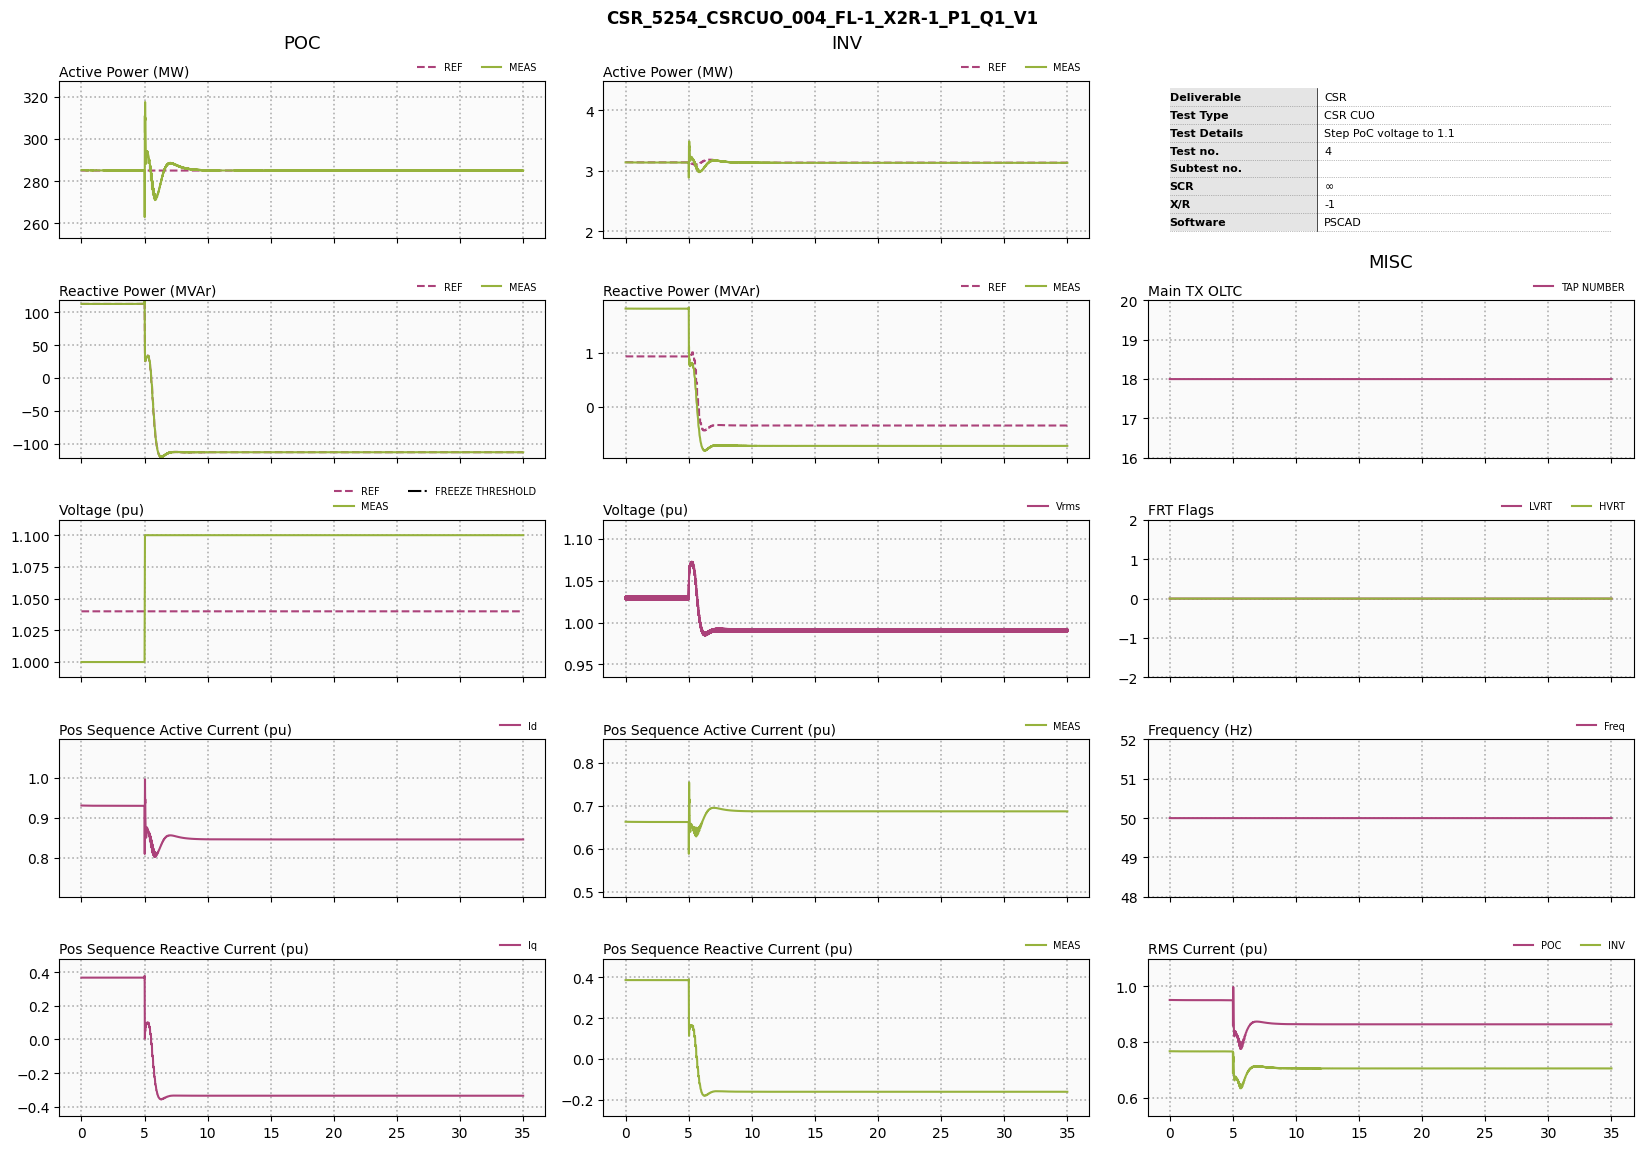
\includegraphics[width=0.7\textwidth]{\analysisdir/pscad/CSR_5254_CSRCUO_004_FL-1_X2R-1_P1_Q1_V1_0.png}
				\caption{HVRT voltage withstand performance - highest terminal voltages}
				\label{fig:s5253-HVRT-AAS}
			\end{figure}
			
			
				
			The ability of the plant and the individual production units to maintain \ac{CUO} can be confirmed through the combination of the reactive capability studies presented in this report, and the chart in Figure \ref{fig:s5254-cuo-summary-pscad}, which shows that the inverter terminal voltages settle within the continuous operating limits prior to any protection or other limiters operating for all \ac{CUO} test cases in Table \ref{tab:s5254-cuo-test-suite}. All test cases have been overlaid on the plot to demonstrate that all inverters settle to within their continuous operating voltage limits for all \ac{CUO} tests without the need for tap changer operation.
			
			The full suite of CUO tests can be viewed in Appendix \ref{Continuous Uninterrupted Operation}.
			
			\begin{figure}[H]
				\centering
				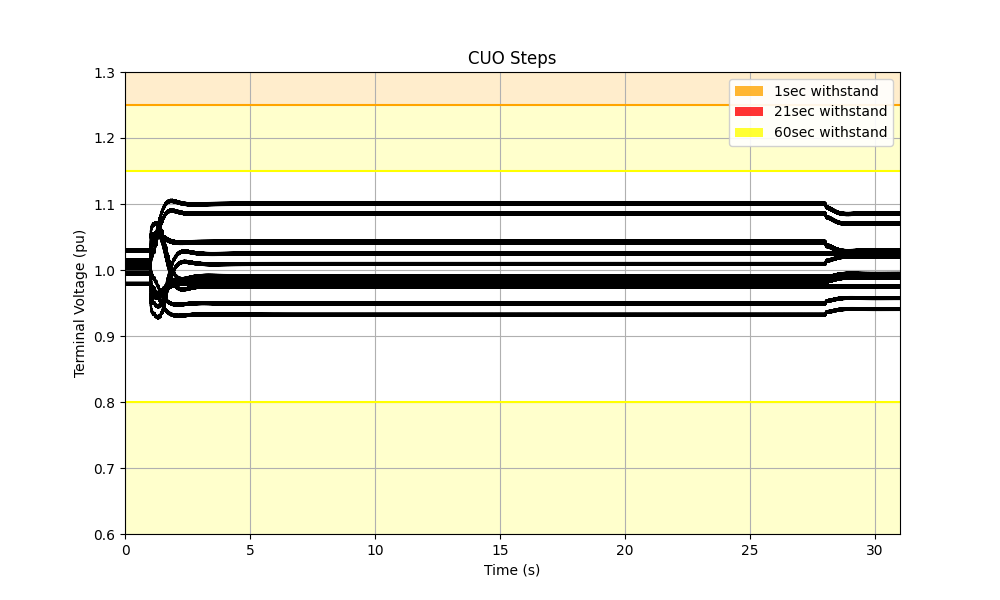
\includegraphics[width=0.9\textwidth]{\analysisdir/pscad/cuo_summary.png}
				\caption{Inverter CUO performance summary plot (PSCAD)}
				\label{fig:s5254-cuo-summary-pscad}
			\end{figure}
	
			\autoscaledlongtable
				{s5.2.5.4 CUO test suite (PSCAD)}
				{tab:s5254-cuo-test-suite}
				{\projectassetsdir/test-suite-tables/5254-CUO-test-table.csv}
	
	
	\section{[S5.2.5.5] Generating System Response to Disturbances Following Contingency Events}
		\subsection{Proposed Access Standard}
		\textbf{Negotiated Access Standard}
			\begin{tcolorbox}[lightgreenbox]
				For the purposes of this performance standard, a \textbf{fault} includes a fault of the relevant type having a metallic conducting path. 
Fault clearance times for relevant equipment are specified in Table 2.6:

	\begin{table}[H]
	\centering
	\begin{tabular}{|c|p{8cm}|}
		\hline
		\textbf{System} & \textbf Transmission system fault clearance time \\ \hline
		Primary protection system & 100 ms \\ \hline
		Breaker fail protection system & 250 ms \\ \hline
		Automatic reclose equipment & 
		Three-phase auto-reclose with 3-second deadtime and 1 shot \\ \hline
	\end{tabular}
	\caption*{Table 2.6: Protection clearance times in transmission and distribution system}
	\end{table}

\textbf{Single disturbance (reflects clause S5.2.5.5(c) of the NER):}  
Provided that the event is not one that would disconnect the integrated resource system from the power system by removing network elements from service, the integrated resource system and each of its production units will remain in continuous uninterrupted operation for any disturbance caused by:
\begin{enumerate}
	\item A credible contingency event;
	\item A three-phase fault in a transmission system cleared by all relevant primary protection systems;
	\item A two-phase-to-ground, phase-to-phase or phase-to-ground fault in the transmission system cleared in:
	\begin{enumerate}
		\item the longest time expected to be taken for a relevant breaker fail protection system to clear the fault or
		\item if a breaker fail protection system is not installed, the greater of the time specified in Table 2.7;
	\end{enumerate}
\end{enumerate}
		
		\begin{table}[H]
		\centering
		\begin{tabular}{|c|p{8cm}|}
			\hline
			\textbf{Nominal voltage at fault location (kV)} & \textbf{Time (ms)} \\ \hline
			>400 kV & 175 ms \\ \hline
			>250 kV and <400 kV & 250 ms \\ \hline
			>100 kV and <250 kV & 430 ms \\ \hline
			<100 kV & 430 ms \\ \hline
		\end{tabular}
		\caption*{Table 2.7: Fault Clearance Times}
		\end{table}

		and the longest time expected to be taken for all relevant primary protection systems to clear the fault.
\begin{enumerate}
	\setcounter{enumi}{3}
	\item A three-phase, two-phase-to-ground, phase-to-phase or phase-to-ground fault in a distribution network cleared in:
	\begin{enumerate}[label=\roman*]
		\item the longest time expected to be taken for a relevant breaker fail protection system to clear the fault; or
		\item if a breaker fail protection system is not installed, the greater of 430 ms and the longest time expected to be taken for all relevant primary protection systems to clear the fault.
	\end{enumerate}
\end{enumerate}

\textbf{Multiple disturbances (reflects clause S5.2.5.5(d), (s), and (t) of the NER):}  
When assessing multiple disturbances, a fault that is re-established following operation of automatic reclose equipment is counted as a separate disturbance.  
The integrated resource system and each of its production units will remain in continuous uninterrupted operation for a series of up to 15 disturbances within any 5-min period caused by any combination of the events described above where:
\begin{enumerate}
	\item Up to 6 disturbances cause the Connection Point voltage to drop below 50\% of Normal Voltage; 
	\item In parts of the network where three-phase automatic reclosure is permitted, up to two disturbances are three-phase faults, and otherwise up to one three-phase fault where the Connection Point voltage drops below 50\% of Normal Voltage; 
	\item Up to one disturbance is cleared by a breaker fail protection system or similar backup protection system; 
	\item Up to one disturbance causes the Connection Point voltage to vary within the ranges under clause S5.2.5.4(a)(7) and (8) of the NER; 
	\item The minimum clearance from the end of one disturbance and commencement of the next disturbance may be zero milliseconds; and 
	\item All remaining disturbances are caused by faults other than three-phase faults, provided that none of the events would result in:
	\item The islanding of the integrated resource system or cause a material reduction in power transfer capability by removing network elements from service; 
	\item The cumulative time that the Connection Point voltage is lower than 90\% of Normal Voltage exceeding 1,800 milliseconds within any 5-min period; or 
	\item Within any 5-min period, the time integral of the difference between 90\% of Normal Voltage and the Connection Point voltage when the Connection Point voltage is lower than 90\% of Normal Voltage exceeding 1 pu second.
The integrated resource system will not, as a consequence of its connection, cause other generating plant or loads to trip as a result of an event, when they would otherwise not have tripped for the same event.
\end{enumerate}

\textbf{For asynchronous integrated resource systems (reflects clause S5.2.5.5(f)-(i) and (u) of the NER):}  
Subject to any changed power system conditions or energy source availability beyond the Integrated Resource Provider's reasonable control, the integrated resource system, including all operating asynchronous production units (in the absence of a disturbance), in respect of fault types described in clause S5.2.5.5(c)(2) to (4) of the NER, will supply to, or absorb from, the network:

\begin{enumerate}
	\item During the disturbance and maintained until the Connection Point voltage recovers to between 90\% and 110\% of Normal Voltage, to assist the maintenance of power system voltages during the fault:
	\begin{enumerate}
		\item Capacitive reactive current in addition to its pre-disturbance level of at least 2.94\% of the maximum continuous current for each 1\% reduction of the Connection Point voltage below the range of  85\% to 90\% of Normal Voltage up to the maximum continuous current; 
		\item Inductive reactive current in addition to its pre-disturbance level of at least 3.1\% of its maximum continuous current for each 1\% increase of the Connection Point voltage above the range of 110\% to 115\% of Normal Voltage up to its maximum continuous current to maintain its rated apparent power; and

		\item the reactive current response will have a rise time of no greater than 40 ms and a settling time of no greater than 133 ms and will be adequately damped; and
		\item the reactive current contribution is calculated using sequence components
	\end{enumerate}
	\item from 230 ms after clearance of the fault, active power of at least 95\% of the level existing just prior to the fault. 
\end{enumerate}

			\end{tcolorbox}
		\subsection{Assessment Methodology}
		\label{subsec:assessment-method-s5255}
			Assessment of s5.2.5.5 is performed in by applying a variety of different types of faults with different impedances to observe the generating system response and measure characteristics such as settling times and $i_{\text{q}}$ injection performance. 

In PSCAD and PSSE SMIB studies, faults are applied to the connection point (as shown in Figure~\ref{fig:s5255-fault-application-methodology-diagram}) with characteristics that are representative of how real world faults would appear from the generating system's connection point, while in PSSE wide area studies, faults with credible characteristics are applied to the real network assets.

\begin{figure}[H]
	\centering
	\newcommand{\bushere}[3]{% length, text above, text below}
% Optional arguments do nto work in paths
%
% starting point; draw an edge and then two nodes
% save the position
coordinate(tmp)
% go up and do an edge down
++(0,#1) node[anchor=base, font=\footnotesize]{#2} edge[ultra thick] ++(0, {-2*#1})
% edges do not move the current point, go down to position the node
++(0,{-2*#1}) node[below]{#3}
% go back to where we started
(tmp)
}

\ctikzset{sources/fill=gray!20, resistors/fill=gray!20}
\resizebox{0.65\linewidth}{!}{ % Set width to \linewidth
	\begin{tikzpicture}[semithick]% default line width
		% Buses and branches
		\draw (0,0)
		node[left, font=\footnotesize]{Generator} ++(1.5,0) \bushere{1.5}{Connection Point}{} coordinate(poc);
		\draw (poc)
		-- ++ (1,0) to[generic, l={$Z_{\text{grid}}$}, resistors/width=2] ++ (4,0)
		-- ++ (1,0)
		\bushere{1.5}{Infinite Bus}{} coordinate(infinite bus);
		% One load (start from the coord load, go up)
		\ctikzset{bipoles/border margin=0.5}% See manual section 3.1.2
		\draw (infinite bus) -- ++(1,0) node[vsourcesinshape, rotate=90]{} ++(0.5,0) node[right]{$V_{\text{grid}}$};
		\draw (poc) -- ++(-1,0) node[vsourcesinshape, rotate=90]{};
		% Fault
		\draw[red, font=\footnotesize] (poc) ++(0, -0.7) -- ++(0.7,0) -- ++(0,-1) node[ground]{} ++(0.6,0.2) node[]{$Z_{\text{fault}}$};
		
	\end{tikzpicture}
}






	\caption{SMIB fault application methodology}
	\label{fig:s5255-fault-application-methodology-diagram}
\end{figure}

In addition to faults, \ac{TOV} scenarios are studied in PSCAD SMIB by tapping a dummy transformer connected between the point of connection and the grid impedance in order to push the voltage at the point of connection up to a specific value. This allows finer control of the disturbance seen at the point of connection, as the voltage drop across the grid impedance doesn't need to be considered.

In order to assess the impact of the project on the South Australian electrical network, four wide area cases were prepared based on recommendations provided by ElectraNet. Descriptions of the four cases are available in Section \ref{sec:s52512} [S5.2.5.12] Impact on Network Capability. 

%For each case, the interconnector flows are characterised by the below.
%
%\begin{enumerate}
%	\item SA light load - Interconnectors exporting 850 MW. Barker Inlet and Snapper Point in service.
%	\item SA light-medium load - Interconnectors exporting 850 MW. Barker Inlet, Snapper Point, and QPS 5 in service.
%	\item SA medium-high load - Interconnectors importing 750 MW. Barker Inlet, Snapper Point, Pelican unit \#1, and QPS 5 in service.
%	\item SA high load - Interconnectors importing 1,300 MW. Barker Inlet, Snapper Point, Pelican units \#1 and \#2, and QPS 5 in service.
%\end{enumerate}
%
%The interconnectors and corresponding limits applicable to this project have been prepared below.
%
%\begin{table}[H]
%	\centering
%	\begin{tabular}{|c|c|c|}
%		\hline
%		Interconnector & Flow direction & Nominal Capacity (MW) \\ \hline
%		Heywood (VIC-SA) & Towards VIC & 550 \\ \hline
%		Heywood (VIC-SA) & Towards SA & 600 \\ \hline
%		PEC (SA-VIC-NSW) & Towards NSW & 800 \\ \hline
%		PEC (SA-VIC-NSW) & Towards SA & 800 \\ \hline
%		Murraylink (VIC-SA) & Towards Vic & 200 \\ \hline
%		Murraylink (VIC-SA) & Towards SA & 220 \\ \hline
%	\end{tabular}
%	\caption{Interconnector flows applicable to this project}
%	\label{tab:case-interconnector-flow}
%\end{table}
%The list of faults evaluated in WAN studies was limited to those studied as part of R0 - as directed by ElectraNet.
%
%Faults were carried out using AEMO's OPDMS snapshots, which incorporated nearby generation and the generator SMIB model, and evaluated performance of the generator for disturbances on the wide area network. A variety of faults were tested, including:
%
%\begin{itemize}
%	\item Three-phase-to-ground faults with circuit breaker failure clearance times
%	\item Two-phase-to-ground faults
%\end{itemize}
			
			All SMIB assessments for this clause have been performed in PSCAD and all wide-area assessments have been performed in PSS/E.
			
		\subsection{Results}
		
			\subsubsection{SMIB studies}
			The faults evaluated to identify the Negotiated Access Standard performed in the SMIB studies were the \ac{DMAT} \cite{pscad-dmat-report} balanced and unbalanced fault set, including tests carried out at maximum and minimum POC SCR. These have been evaluated with the integrated resource system in both charging and discharging mode. The plant was not able to achieve an automatic access standard for this clause, and a technical note is provided to support the negotiated performance standard requested. \cite{fault-performance-memo}
			
			452 faults and overvoltage events were analysed as part of this negotiated standard, which included.
			\begin{itemize}
				\item DMAT balanced faults (section 3.2.4)
				\item DMAT unbalanced faults (section 3.2.5)
				\item DMAT "POC SCR" faults (section 3.2.19)
				\item CSR TOV tests (DMAT tests were not sufficient to cause entry into FRT mode)
			\end{itemize}
			
			Fault study results can be reviewed in DMAT appendices B, C and M. TOV study results can be viewed in Appendix \ref{Temporary Over-Voltage Tests}.
		
			For subclauses pertaining to capacitive and inductive current contribution, figure \ref{fig:5255-pscad-diqdv-poc} shows the amount of $i_{\text{q}}$ injection at the point of connection to the change in connection point voltage across all faults studied. It can be read as follows:
			\begin{itemize}
				\item Grey circles indicate that the generating system is supplying more than the \textit{maximum continuous current} of the generating system\footnote{The current associated with maximum active power and maximum reactive power while at 1.0pu voltage.}, which automatically fulfils the GPS requirement for reactive current injection, regardless of the additional $i_{\text{q}}$ injected.
				\item Red markers indicate the amount of additional $i_{\text{q}}$ injected for a particular fault. For compliance, the marker should be above the access standard characteristic (for faults) or below the characteristic (for \ac{TOV} tests).
			\end{itemize}
			
			\begin{figure}[H]
				\centering
				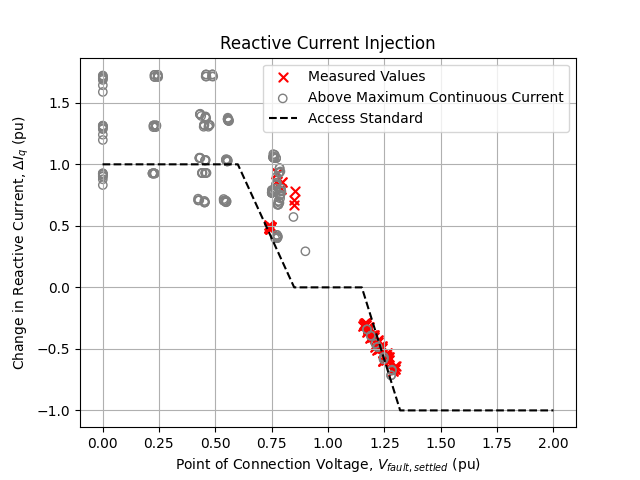
\includegraphics[width=0.8\textwidth]{\analysisdir/pscad/diqdv_characteristic.png}
				\caption{POC Reactive Current Injection Performance}
				\label{fig:5255-pscad-diqdv-poc}
			\end{figure}
			

			 All faults tested were able to contribute the maximum required current consistent with an automatic access standard at the point of connection. The current output at the point of connection was either saturated, or in excess of the requirement for capacitive contribution. The plant performance standard has therefore been set at 4\%.
			 
			\textbf{Iq rise and settling times}
			
			Rise and settling times were in excess of those required to meet the automatic access standard. Behaviour of the plant under shallow fault conditions, particularly when charging, resulted in longer rise and settling times than the requirement. The aggregate performance of the plant with regards to reactive current rise and settling times is shown in Figure \ref{fig:iq-rise-settle-pscad}.
			
			\begin{figure}[H]
				\centering
				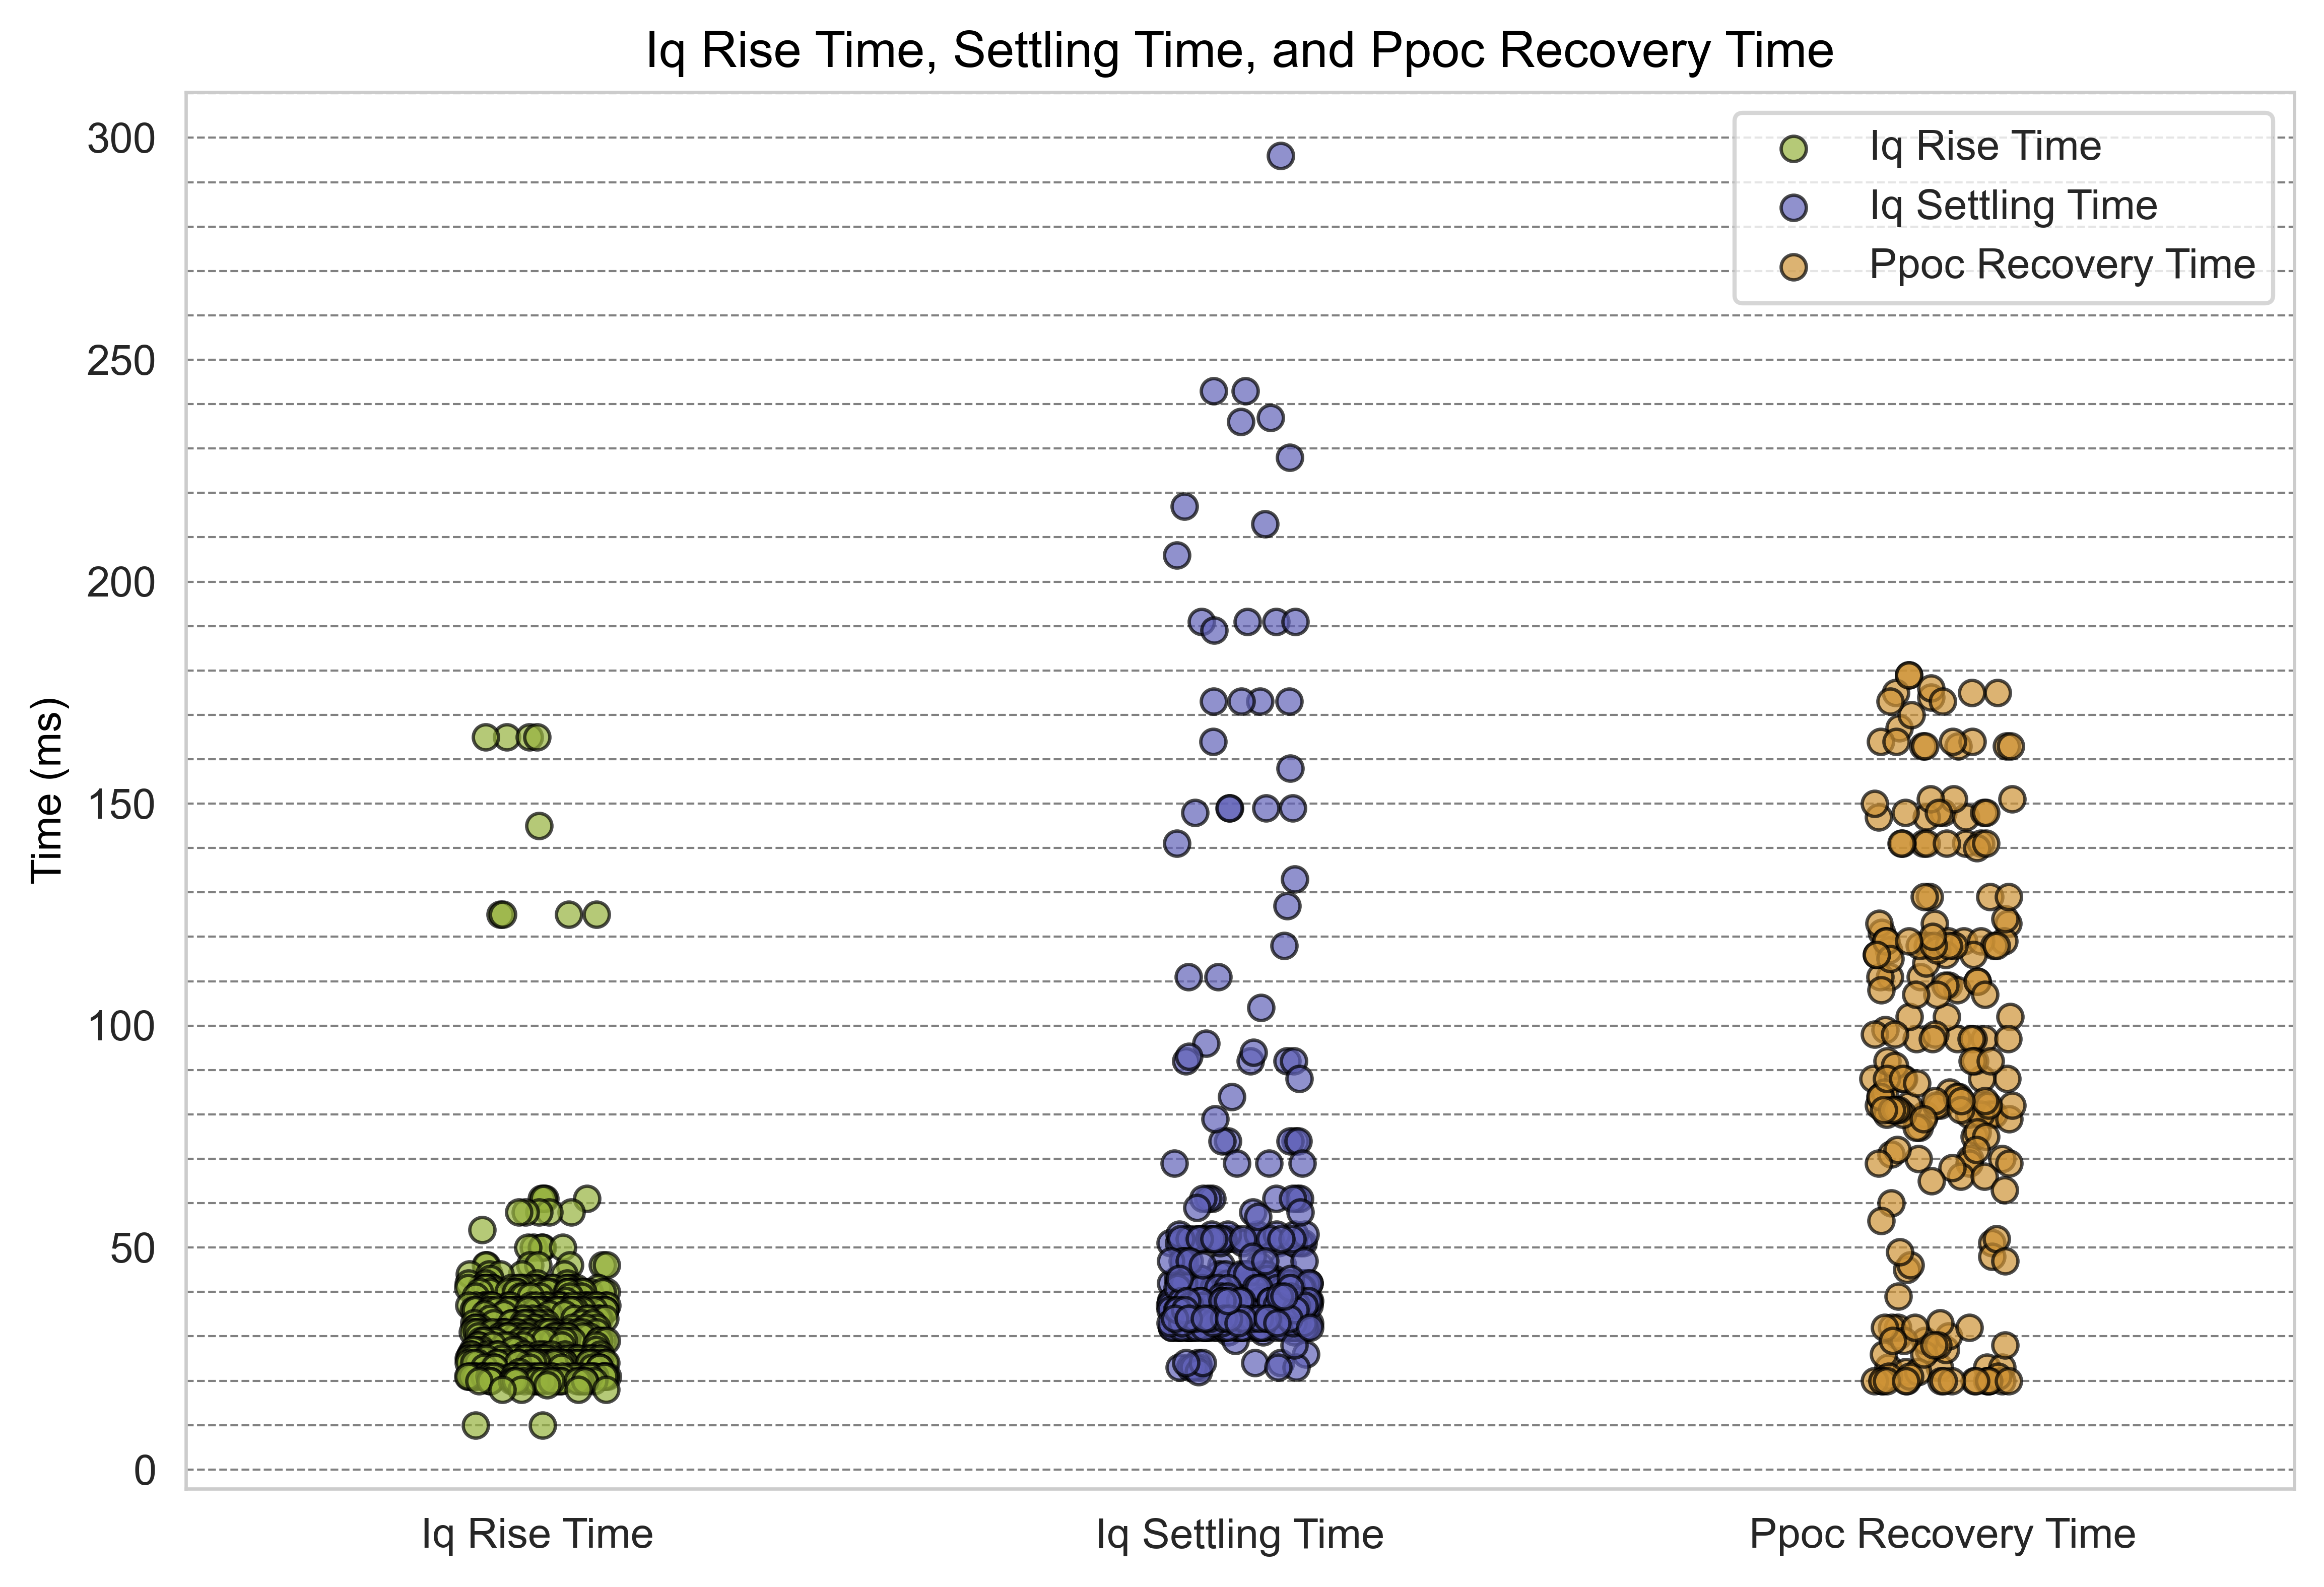
\includegraphics[width=0.9\textwidth]{\analysisdir/pscad/separated_stripplot_with_optimized_gridlines.png}
				\caption{Reactive current rise and settling time performance}
				\label{fig:iq-rise-settle-pscad}
			\end{figure}
			
			Figure \ref{fig:iq-rise-settle-pscad} shows that approximately 1/4 of faults are responsible for rise and settling times in excess of the automatic access standard requirements. The behaviour of these faults were investigated to determine the cause of these increased times. Of these faults, the longest settling were shallow faults that did not cause entry into FRT. These faults are visible in the above Figure, but have been excluded from the GPS as they do not represent settling time of a reactive current response. 
			
			Aside from these faults, the longest rise times and settling times occurred due to a sustained increase in reactive current throughout the fault. An example of this behaviour is shown in Figure \ref{fig:longest-settling-time}, which shows the performance of the longest settling time observed across a fault.
			
			\begin{figure}[H]
				\centering
				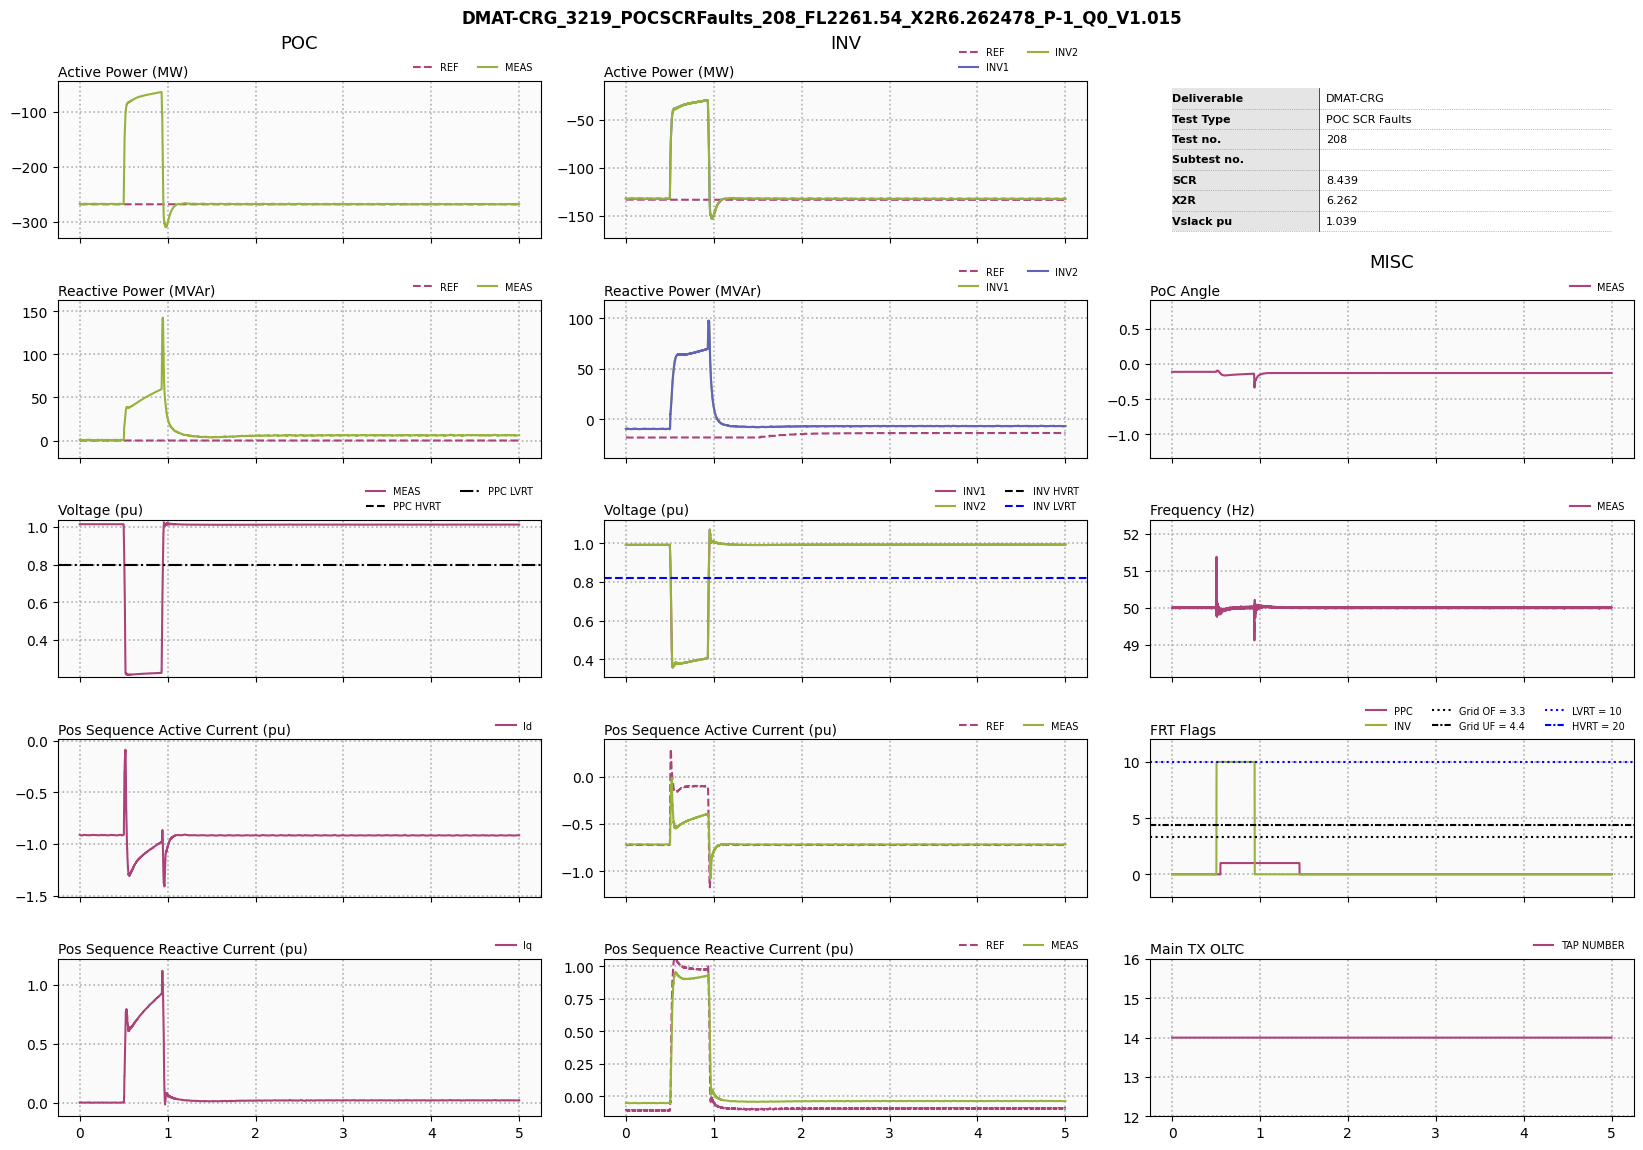
\includegraphics[width=0.9\textwidth]{\analysisdir/pscad/DMAT-CRG_3219_POCSCRFaults_208_FL2261.54_X2R6.262478_P-1_Q0_V1.015.png}
				\caption{Reactive current rise and settling time performance}
				\label{fig:longest-settling-time}
			\end{figure}
			
			It can be seen that although the BESS response at its inverter terminals settles quickly within a range, the reactive current measured at the point of connection continues to move throughout the fault. This measurement appears to be influenced by the PoC angle, which is driven in line with the reduced active power absorbed by the BESS throughout the fault. This behaviour, although increasing calculated rise and settling times significantly, is not considered to be undesirable or problematic for the power system as an undamped response would be. 
			
			It is noted, that if these faults where such behaviour occurred were excluded from analysis, the maximum  settling time would be \textbf{94 ms}, and maximum rise time would be \textbf{50 ms}, however for the purpose of the performance standard, these faults have been included to set a maximum rise time of \textbf{170 ms} and a settling time of \textbf{220 ms}.
			
			\textbf{Active power recovery}
			
			For the subclause pertaining to active power recovery time, it was not possible to achieve a recovery time of 100 ms for the majority of faults tested. The worst performance during this fault was seen for recovery to extremely low setpoints i.e. 5\% of rated output, which can be challenging to recover to, compared to operating near rated power.
			
			To avoid prolonging the recovery time recorded in the GPS, the automatic access standard has been set based on recovery to 95\% of the active power of the BESS, or within 10 MW of the existing setpoint, whichever is lower, to avoid setting a standard based on prolonged fault recovery to extremely low setpoints. As a grid-forming plant, the inverters are sensitive to angle changes under fault conditions, and therefore tuning this behaviour out through settings changes is difficult to accomplish. The largest active power recovery time observed for a fault has been used to set the suggested Negotiated Performance Standard of \textbf{180 ms}.
		

			\textbf{Temporary overvoltage}
			
			The list of \ac{TOV} studies performed can be seen in Table \ref{tab:s5255-tov-test-suite-pscad}. The DMAT tests were not chosen for evaluation with respect to this clause, as they did not consistently cause the converters to enter into fault ride thorough mode, meaning that they were not under reactive current control, but rather reactive power control. An alternative set of tests were performed to test compliance with this clause, which caused higher overvoltages which allowed the converters to enter \ac{FRT} mode.
			
			{
				\autoscaledlongtable
				{ToV tests}
				{tab:s5255-tov-test-suite-pscad}
				{\projectassetsdir/test-suite-tables/CSR-TOV-test-table.csv}
			}
			
			\begin{figure}[H]
				\centering
				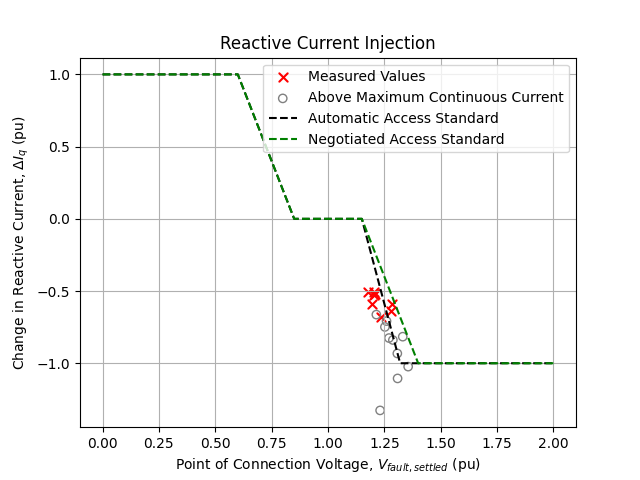
\includegraphics[width=0.9\textwidth]{\analysisdir/pscad/diqdv_characteristic_tov.png}
				\caption{ToV performance}
				\label{fig:iq-tov}
			\end{figure}
			
			Analysis of the studies undertaken showed that the plant had two tests which did not meet an automatic access standard, absorbing 4.34\% iq per 1\% increase in voltage at the point of connection above 115\%. Higher gain in the HVRT threshold, although achievable through plant settings, was not considered to be desirable when operating the plant at low SCR, as entering HVRT with a high gain could lead to re-triggering or voltage collapse. Therefore, the performance standard has been set at 4\%. 
			
			The performance of the \ac{IRP} with regards to fault ride through and ToV does not meet the automatic access standard of this clause. An explanation of the tuning process, and the justification of the decisions made for to propose this standard is given in a technical memorandum. \cite{fault-performance-memo}
			
			\textbf{MFRT}
			
			The multiple fault ride through performance of the model was assessed by the DMAT MFRT tests, visible in DMAT appendix D. The model was capable of remaining in \ac{CUO} throughout the suite of tests applied in all cases. Sungrow have also provided a manufacturer certification of performance under MFRT conditions. \cite{sungrow-mfrt}


		\subsubsection{WAN studies}

		The contingencies considered for wide area network assessment have been summarised in the tables below, and are consistent with the document provided by AEMO as part of the pre-application scope of works. \cite{wan-contingency-list} As per AEMO's instructions, the highest and lowest load study cases for Victoria have been considered, which corresponded to the autumn high and autumn low OPDMS snapshots. The VNI and Heywood interconnector flows in the "low load" cases developed were modified to correspond to exceed 70\% loading on each case, to develop "Import" and "Export" conditions for Victoria, as per the AEMO Interconnector Capabilities document. \cite{aemo-interconnector-advice}  The BESS was dispatched at rated active power discharging in the high load and low load export cases, and at rated active power charging in the low load import case. A range of faults and tripping of network elements have been considered.
		
		{
			\fontsize{5}{7}\selectfont
			\autoscaledlongtable
				{Wide area studies test suite - faults (PSSE)}
				{tab:wide-area-contingencies}
				{report-assets/analysis/psse-wan/WAN_tests/contingencies.csv}
		}
		
		{
			\fontsize{9}{7}\selectfont
			\autoscaledlongtable
			{Wide area studies test suite - trips (PSSE)}
			{tab:wide-area-contingencies-2}
			{report-assets/analysis/psse-wan/WAN_tests/contingencies_2.csv}
		}
		
		The results for each case can be evaluated in Appendix \ref{Autumn High - Wide Area Network Contingency Results}-\ref{Autumn Low Import - Wide Area Network Contingency Results}.
		
		While overall good performance was observed from the plant across the range of contingencies studied, one issue occurred under the most significant fault tested across multiple scenarios - a local fault disconnecting the Learmonth Terminal Station from Ballarat Terminal Station, which was cleared at each end of the 220 kV line connecting the stations. The close up fault on the generator is significant both due to the severity of the drop in retained voltage, but also due to the impact that this trip has on network flows and system strength in the area. The tripping of the existing line results in the activation of the GFT (generator fast tripping) scheme, with other generation on the line disconnected.
		
		This fault was modelled as a bolted fault at 1\% distance from Learmonth Terminal Station. In addition to the fault, generation was disconnected as per the GFT scheme referenced in the AEMO document \cite{gft-scheme-doc}, with the following generators disconnected following fault application:
		
		\begin{itemize}
			\item Waubra wind farm
			\item Ararat wind farm
			\item Crowlands wind farm
			\item Bulgana Green Power Hub wind farms
			\item Murra Warra wind farms 1 and 2
		\end{itemize}
		
		Under this contingency, the BESS loses stability following fault clearance and disconnection of generators as per the GFT scheme. The performance of the BESS in the Autumn High case is shown in \ref{fig:bess-instability}.
		
		\begin{figure}[H]
			\centering
			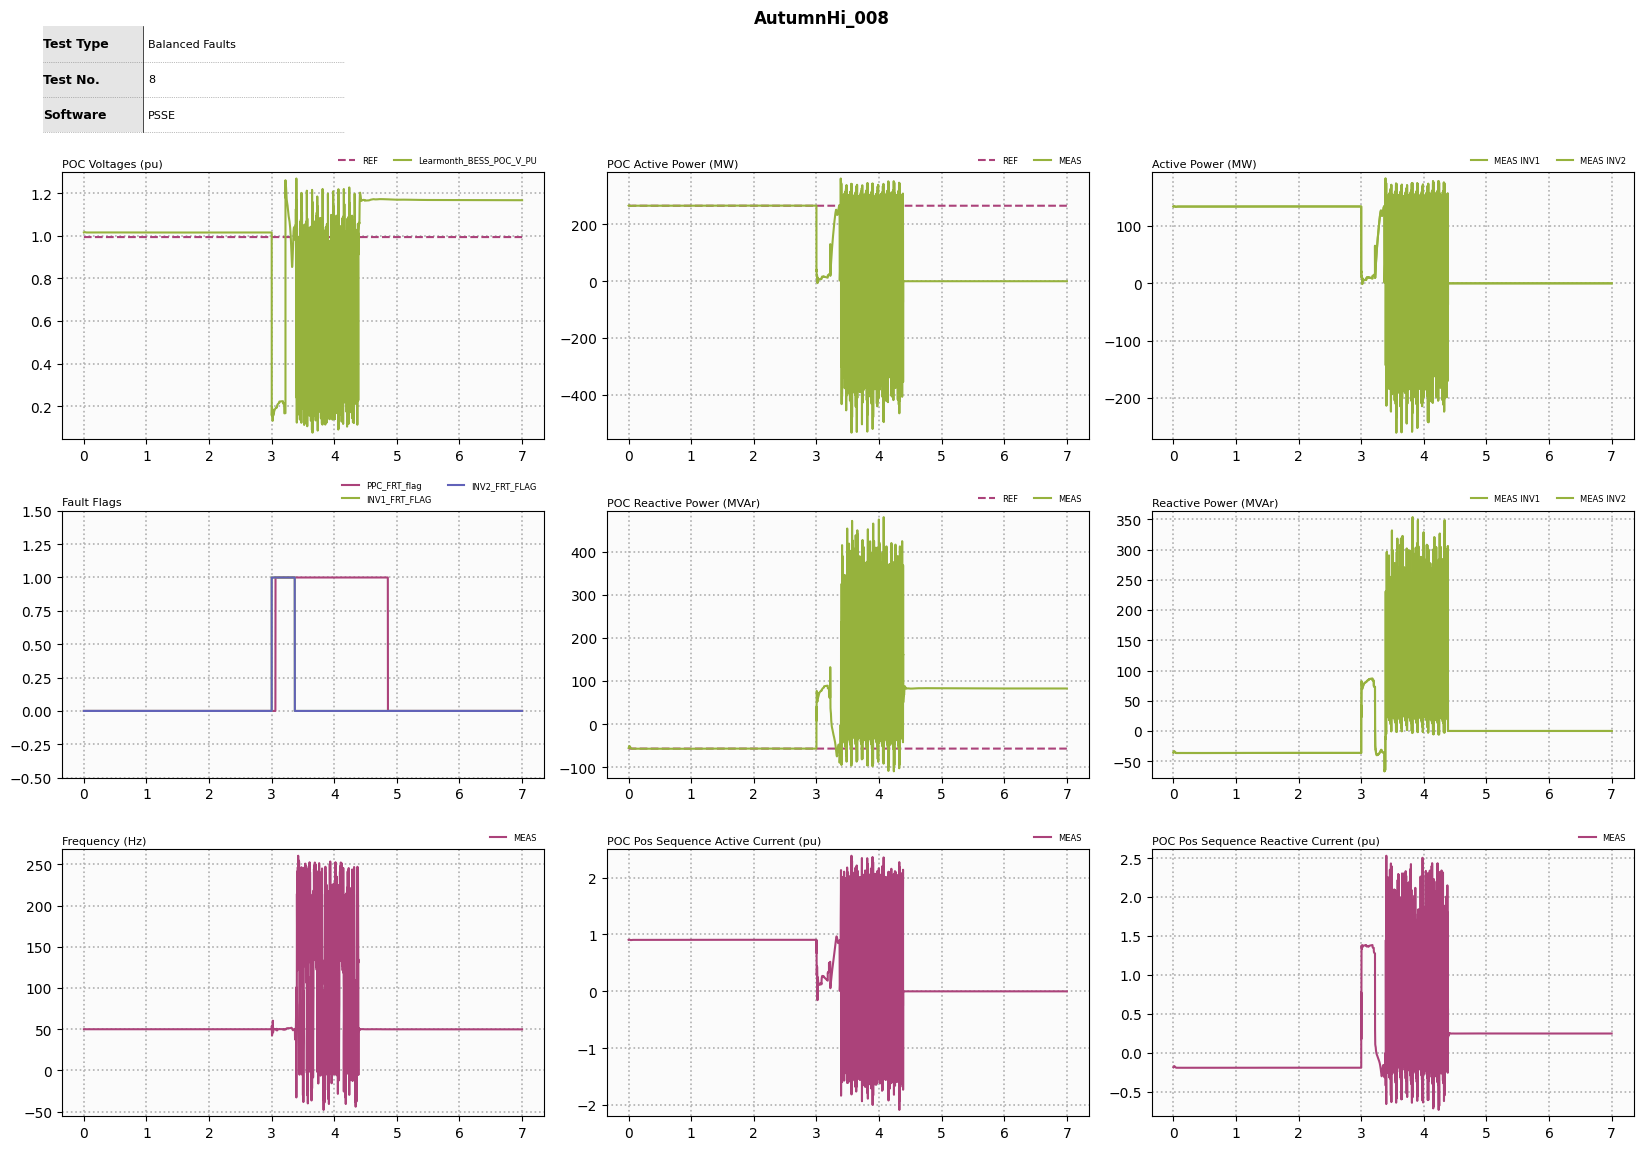
\includegraphics[width=0.9\textwidth]{\analysisdir/pscad/AutumnHi_008gen.png}
			\caption{Autumn high - BESS instability}
			\label{fig:bess-instability}
		\end{figure}
		
		This fault reduces the SCR at the BESS terminals significantly more than any other event, particularly in the low demand cases where synchronous fault level is at a minimum. 
		
		The performance of the BESS under this event has been investigated with the converter OEM Sungrow, who have provided a technical note for review by AEMO. Sungrow have advised that the ability of PSSE to represent the response of a voltage source converter is limited under low SCR conditions, and that the response of the model to this fault should be investigated using a wide area PSCAD model. \cite{sungrow-response-learmonth-fault}
		
		It is therefore suggested that the performance of the BESS and ability to operate under these conditions is set by the performance of PSCAD model, which has demonstrated low SCR operation in a SMIB environment.

			
	\section{[S5.2.5.6] Quality of Electricity Generated and Continuous Uninterrupted Operation}
	\subsection{Proposed Access Standard}
	\textbf{Minimum Access Standard}
		\begin{tcolorbox}[lightgreenbox]
			The integrated resource system and each of its operating production units and reactive plant, will not disconnect from the power system for voltage fluctuation, harmonic voltage distortion and voltage unbalance at the Connection Point within the levels specified:
\begin{enumerate}
	\item For voltage fluctuations at the Connection Point, in the "compatibility levels" set out in Table 1 of AS/NZS 61000.3.7:2001.
	\item For harmonic voltage distortion at the Connection Point, in the "compatibility levels" defined in Table 1 of AS/NZS 61000.3.6:2001.
	\item For a negative sequence voltage at the Connection Point, in Table S5.1a.1 of the NER and shown in Table 2.8:
\end{enumerate}

\begin{table}[H]
	\centering
	\resizebox{\textwidth}{!}{%
		\begin{tabular}{|c|c|c|c|c|}
			\hline
			\textbf{Nominal Supply Voltage (kV)} & \textbf{No Contingency Event} & \multicolumn{2}{|c|}{\textbf{Credible Contingency Event}} & \textbf{General} \\ \hline
			& \textbf{30-Minute Average} & \textbf{30-Minute Average} & \textbf{10-Minute Average} & \textbf{1-Minute Average} \\ \hline
			> 100 & 0.5\% & 0.7\% & 1.0\% & 2.0\% \\ \hline
		\end{tabular}%
	}
	\caption*{Table 2.8: Negative Sequence Voltages}
\end{table}

		\end{tcolorbox}
	\subsection{Assessment Methodology}
		s5.2.5.6 is not assessed through simulation software. Compliance with this clause is confirmed through a letter supplied by the converter OEM. Sungrow have prepared a NER compliance report which covers the ability of their converters to meet the automatic access standard for S5.2.5.6.\cite{sungrow-s5256-compliance-letter}
	
	\section{[S5.2.5.7] Partial Load Rejection}
	\subsection{Proposed Access Standard}
	\textbf{Automatic Access Standard}
		\begin{tcolorbox}[lightgreenbox]
			For the purposes of this performance standard:
\begin{itemize}
	\item \textbf{Minimum generation} means the minimum sent-out generation for continuous stable operation, $P_{\text{MIN}} = 0$ MW.
\end{itemize}

The integrated resource system is capable of continuous uninterrupted operation during and following a power system load reduction of 30\% from its pre-disturbance level or equivalent impact from separation of part of the power system in less than 10 s, provided that the loading level remains above $P_{\text{MIN}}$.

		\end{tcolorbox}
	\subsection{Assessment Methodology}
		\ac{PLR} tests assess the ability of the generator to ride through the angle change associated with a loss of a significant percentage of the load they are supplying into. While more relevant for traditional synchronous machines supplying the majority of the load to large load centres or industrial customers, an analogous \ac{PLR} test can also be performed in SMIB.

To perform this test, a load equivalent to 30\% of the maximum capacity of the generating system is attached at the connection point and the appropriate $V_{\mathrm{grid}_{\mathrm{initial}}}$ is  identified to achieve $V_{\mathrm{POC}_{\mathrm{initial}}}$ given the required initial $P_{\mathrm{POC}}$, $Q_{\mathrm{POC}}$, SCR and X/R conditions, noting that 30\% of the power flow is no longer being transferred to the slack bus. 

The test is then performed by initialising the system with the load in service, then switching it out of service at the intended disturbance time for the remainder of the simulation, as shown in Figure~\ref{fig:smib-plr-diagram}.


\begin{figure}[h]
	\centering
	\newcommand{\bushere}[3]{% length, text above, text below}
% Optional arguments do nto work in paths
%
% starting point; draw an edge and then two nodes
% save the position
coordinate(tmp)
% go up and do an edge down
++(0,#1) node[anchor=base, font=\footnotesize]{#2} edge[ultra thick] ++(0, {-2*#1})
% edges do not move the current point, go down to position the node
++(0,{-2*#1}) node[below]{#3}
% go back to where we started
(tmp)
}

\ctikzset{sources/fill=gray!20, resistors/fill=gray!20}
\resizebox{0.65\linewidth}{!}{ % Set width to \linewidth
\begin{tikzpicture}[semithick]% default line width
	% Buses and branches
	\draw (0,0)
	node[left, font=\footnotesize]{Generator} ++(1.5,0) \bushere{1.5}{Connection Point}{} coordinate(poc);
	\draw (poc)
	-- ++ (1,0) to[generic, l={$Z_{\text{grid}}$}, resistors/width=2] ++ (4,0)
	-- ++ (1,0)
	\bushere{1.5}{Infinite Bus}{} coordinate(infinite bus);
	% One load (start from the coord load, go up)
	\ctikzset{bipoles/border margin=0.5}% See manual section 3.1.2
	\draw (infinite bus) -- ++(1,0) node[vsourcesinshape, rotate=90]{} ++(0.5,0) node[right]{$V_{\text{grid}}$};
	\draw (poc) -- ++(-1,0) node[vsourcesinshape, rotate=90]{};
	% Capacitor
	\draw[red](poc) ++(0, -0.7) -- ++(0.7,0) -- ++(0,-0.5) to[R] ++(0,-1) node[ground]{};
	
\end{tikzpicture}
}





	\caption{PLR test application methodology}
	\label{fig:smib-plr-diagram}
\end{figure}
		
		All assessments for this clause have been performed in PSCAD.
		
	\subsection{Results}
	
	\subsubsection{SMIB studies}
	
	Due to the limited number of \ac{PLR} tests and the clause not introducing specific performance characteristics associated with the \ac{PLR} response, each simulation is reviewed manually for stability and \ac{CUO}. The test suite assessed can be found in Table \ref{tab:s5257-test-suite-pscad}. Results can be reviewed in full in Appendix \ref{Partial Load Rejection Tests}.
	
	{
		\fontsize{9}{11}\selectfont
		\autoscaledlongtable
		{s5.2.5.7 partial load rejection test suite (PSCAD)}
		{tab:s5257-test-suite-pscad}
		{\projectassetsdir/test-suite-tables/5257-test-table.csv}
	}
	
	\subsubsection{WAN studies}
	
	A partial load rejection event was tested in the NEM in line with \ref{tab:wide-area-contingencies} which shows the APD potline load was tripped - disconnecting >200 MW of load from the NEM in Victoria per case. This test was carried out in all cases studied.
	
	\subsubsection{Conclusion}
	
	The integrated resource system was able to remain in continuous uninterrupted operation for every partial load rejection event studied in both a SMIB and wide area environment. An automatic access standard has been proposed for this clause.
	
	
	\section{[S5.2.5.8] Protection of Generating Systems from Power System Disturbances}
	\subsection{Proposed Access Standard}
	\textbf{Minimum Access Standard}
		\begin{tcolorbox}[lightgreenbox]
			\begin{enumerate}[label=(\alph*)]
	\item Subject to paragraphs (b) and (e) where the integrated resource system or any of its production units that is required by the NSP, Generator or Integrated Resource Provider to be automatically disconnected from the power system in response to abnormal conditions arising from the power system, the relevant protection system or control system does not disconnect the integrated resource system  for:
	\begin{enumerate}[label=(\roman*)]
		\item conditions for which it must remain in continuous uninterrupted operation; or
		\item conditions it must withstand under the NER.
	\end{enumerate}
	\item The integrated resource system has facilities to automatically and rapidly reduce its generation:
	\begin{enumerate}[label=(\roman*)]
		\item in proportion to the difference between the frequency at the Connection Point and a level nominated by AEMO (not less than the upper limit of the operational frequency tolerance band) such that the generation is reduced, by at least half, within 3 s of the frequency reaching the upper limit of the extreme frequency excursion tolerance limits.
	\end{enumerate}
	\item The integrated resource system must be automatically disconnected by a local or remote control scheme whenever the part of the network to which it is connected has been disconnected from the national grid and has formed an island that supplies load.
	\item The conditions for which the integrated resource system must trip and must not trip are: TBC.
	\item Notwithstanding the performance standards under clauses S5.2.5.3, S5.2.5.4, S5.2.5.5, S5.2.5.6 and S5.2.5.7 of the NER the integrated resource system may be automatically disconnected from the power system under any of the following conditions s:
	\begin{enumerate}[label=(\arabic*)]
		\item in accordance with the ancillary services agreement dated [insert date] between the Integrated Resource Provider and AEMO for the provision o
		\item where the integrated resource system is automatically disconnected under paragraphs (a), (b), or the performance standard under clause S5.2.5.9 of the NER;
		\item where the integrated resource system is automatically disconnected under the performance standard under clause S5.2.5.10 of the NER; or
		\item in accordance with an agreement between the Integrated Resource Provider and the NSP (including an agreement in relation to an emergency control scheme under clause S5.1.8 of the NER) to provide a service that AEMO agrees is necessary to maintain or restore power system security in the event of a specified contingency event.
		\item Where the integrated resource system is automatically disconnected from the power system via an emergency frequency control scheme (EFCS) in accordance with an EFCS settings schedule as maintained by AEMO and notified to the Integrated Resource Provider from time to time.
	\end{enumerate}

\end{enumerate}

		\end{tcolorbox}
	\subsection{Assessment Methodology}
		Clause s5.2.5.8(b) is assessed without any additional tests being run, as a frequency ramp to 52.0 Hz is already performed under s5.2.5.11, for which the methodology is described in Section \ref{subsec:s52511-assessment-methodology}. All assessments for this sub-clause have been performed in PSCAD.
		
		Compliance to other elements of the clause are not confirmed through power system analysis, and will be confirmed at detailed design stage of the project.
		

	\subsection{Results}
	Table \ref{tab:s5258-results-pscad} shows the results of the rapid active power reduction tests. As shown, the generating system is able to reduce its active power by half within 3 seconds of the connection point frequency reaching 52.0Hz.
	
	Under all cases where operating with sufficient headroom to reduce active power, the plant was capable of reducing its output by 50\% before the connection point frequency of 52 Hz was reached, as expected when operating under a 5\% droop setting and with a fast inertial response. The results of these tests can be viewed in the discharging DMAT Appendix H.
	
		{
			\fontsize{9}{11}\selectfont
			\autoscaledlongtable
			{s5.2.5.8 rapid active power reduction results (PSCAD)}
			{tab:s5258-results-pscad}
			{report-assets/analysis/pscad/Active Power Reduction Analysis.csv}
		}


	\section{[S5.2.5.11] Frequency Control}
	\subsection{Proposed Access Standard}
	\textbf{Automatic Access Standard}
		\begin{tcolorbox}[lightgreenbox]
			For the purposes of this performance standard:
\begin{itemize}
	\item \textit{‘Maximum operating level’} = 285 MW.
	\item \textit{‘Minimum operating level’} = -285 MW.
	\item \textit{‘Droop’} means, in relation to frequency response mode, the percentage change in power system frequency as measured at the Connection Point, divided by the percentage change in power transfer of the integrated resource system, expressed as a percentage of the maximum operating level of the integrated resource system.  Droop must be measured at frequencies that are outside the deadband and within the limits of power transfer.
	\item Power system frequency is measured at the Connection Point.
\end{itemize}

\begin{enumerate}[label=(\arabic*)]
	\item an integrated resource system, to the extent it comprises production units, must be capable of operating in frequency response mode such that it automatically provides a proportional:
	\begin{enumerate}[label=(\roman*)]
		\item decrease in power transfer to the power system, with a continuous shift from one to the other mode, in response to a rise in the frequency of the power system as measured at the connection point accompanied by a smooth change in bidirectional unit operating mode between production and consumption; and
		\item increase in power transfer to the power system in response to a fall in the frequency of the power system as measured at the connection point accompanied by a smooth change in bidirectional unit operating mode between production and consumption, 
	\end{enumerate}
	sufficiently rapidly and sustained for a sufficient period for the Integrated Resource Provider (as relevant) to be in a position to offer measurable amounts of all market ancillary services for the provision of power system frequency control.
	\item Nothing in paragraph (2) or (3) requires the integrated resource system to operate below its minimum operating level in response to a rise in power system frequency, or above its maximum operating level in response to a fall in power system frequency.  
	\item The change in power transfer to the power system will occur with no delay beyond that required for stable operation, or inherent in the plant controls, once power system frequency leaves a deadband around 50 Hz.
	\item The integrated resource system’s:
	\begin{enumerate}[label=(\roman*)]
		\item deadband can be set within the range of 0 to ± 1.0 Hz ; and
		\item droop can be set within the range of 2\% to 10\%, droop has been set to 5\%.
	\end{enumerate}
	\item Each control system used to satisfy this performance standard is adequately damped.
	\item The amount of relevant market ancillary service for which the plant is registered will not exceed the amount that would be consistent with this performance standard. 
\end{enumerate}

		\end{tcolorbox}
	\subsection{Assessment Methodology}
		\label{subsec:s52511-assessment-methodology}
		To test the frequency droop controller, $F_{\mathrm{grid}}$ is driven with a time-series signal $F_{\mathrm{grid}_{\mathrm{1}}}, F_{\mathrm{grid}_{\mathrm{2}}}, F_{\mathrm{grid}_{\mathrm{3}}}, \dots, F_{\mathrm{grid}_{\mathrm{n}}}$, as shown in Figure~\ref{fig:s52511-methodology}. The active power through the connection point is expected to change by an amount that is proportional to the change in frequency, subject to active power limits and available input power\footnote{Note that while not addressed in this document, the \ac{DMAT} reports show the behaviour of the frequency controller when limited by available input power.}, in line with the agreed droop gain.


\begin{figure}[H]
	\centering
	\newcommand{\bushere}[3]{% length, text above, text below}
% Optional arguments do nto work in paths
%
% starting point; draw an edge and then two nodes
% save the position
coordinate(tmp)
% go up and do an edge down
++(0,#1) node[anchor=base, font=\footnotesize]{#2} edge[ultra thick] ++(0, {-2*#1})
% edges do not move the current point, go down to position the node
++(0,{-2*#1}) node[below]{#3}
% go back to where we started
(tmp)
}

\ctikzset{sources/fill=gray!20, resistors/fill=gray!20}
\resizebox{\linewidth}{!}{ % Set width to \linewidth
	\begin{tikzpicture}[semithick]% default line width
		% Buses and branches
		\draw (0,0)
		node[left, font=\footnotesize]{Generator} ++(1.5,0) \bushere{1.5}{Connection Point}{} coordinate(poc);
		\draw (poc)
		-- ++ (1,0) to[generic, l={$Z_{\text{grid}}$}, resistors/width=2] ++ (4,0)
		-- ++ (1,0)
		\bushere{1.5}{Infinite Bus}{} coordinate(infinite bus);
		% One load (start from the coord load, go up)
		\ctikzset{bipoles/border margin=0.5}% See manual section 3.1.2
		\draw (infinite bus) -- ++(1,0) node[vsourcesinshape, rotate=90]{} coordinate(vgrid) ++(0.5,0) node[right]{$V_{\text{grid}}$};
		\draw (poc) -- ++(-1,0) node[vsourcesinshape, rotate=90]{};
		% Fault
		\draw[blue, font=\footnotesize, <-] (vgrid) ++(0, -0.5) -- ++(0, -0.5) -- ++(0.5,0) node[right]{$F_{\mathrm{grid}_{\mathrm{1}}}, F_{\mathrm{grid}_{\mathrm{2}}}, F_{\mathrm{grid}_{\mathrm{3}}}, \dots, F_{\mathrm{grid}_{\mathrm{n}}}$};
		
	\end{tikzpicture}
}






	\caption{Frequency droop controller testing methodology}
	\label{fig:s52511-methodology}
\end{figure}
		
		All assessments for this clause have been performed in PSCAD.
		
	\subsection{Results}
	The tests performed for this clause have been presented in Table \ref{tab:s52511-frequency-controller-test-suite-pscad}. To confirm the compliance of the generating system to the configured droop characteristic, the steady-state change in active power has been plotted against the associated change in frequency in Figure \ref{fig:52511-frequency-droop-validation-pscad} for all simulations that were run for this clause. The markers on the plot can be understood as follows:
	
	\begin{itemize}
		\item Grey circles indicate that the active power controller reached saturation (either due to it already being saturated or by supplying/reducing so much active power that it reached saturation), which automatically fulfils the GPS requirement for frequency control.
		\item Red markers indicate the amount of active power transfer increase or decrease for a particular frequency disturbance. For compliance, the marker should be on the access standard characteristic.
	\end{itemize}
	
	To avoid interference with the plant inertial response, which will temporarily dominate the response of the plant frequency controller for extremely large frequency deviations, the response of the plant frequency controller was tested for a range of small frequency deviations at the point of connection, which would not cause the plant to exceed its rated active power. The results show a strong alignment to the agreed frequency droop control and, hence, compliance to s5.2.5.11.
	
	\begin{figure}[H]
		\centering
		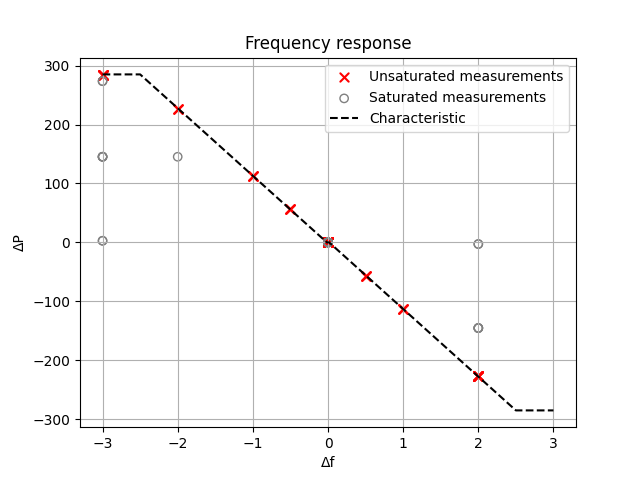
\includegraphics[width=0.7\textwidth]{\analysisdir/pscad/dpdf_characteristic.png}
		\caption{s5.2.5.11 frequency droop characteristic validation (PSCAD)}
		\label{fig:52511-frequency-droop-validation-pscad}
	\end{figure}
	
	A list of tests carried out in both charging and discharging mode for this clause are shown in Tables \ref{tab:s52511-frequency-controller-test-suite-pscad} and \ref{tab:s52511-frequency-controller-test-suite-pscad-crg}. These test results can be viewed in the PSCAD DMAT Appendix P for both charging and discharging conditions.
	
	{
		\fontsize{11}{13}\selectfont
		\autoscaledlongtable
		{s5.2.5.11 frequency droop controller test suite - discharging mode (PSCAD)}
		{tab:s52511-frequency-controller-test-suite-pscad}
		{\projectassetsdir/test-suite-tables/3212-Fgrid-12-test-table.csv}
	}
	
		{
		\fontsize{11}{13}\selectfont
		\autoscaledlongtable
		{s5.2.5.11 frequency droop controller test suite - charging mode (PSCAD)}
		{tab:s52511-frequency-controller-test-suite-pscad-crg}
		{\projectassetsdir/test-suite-tables/3212-Fgrid-12-CRG-test-table.csv}
	}

	\section{[S5.2.5.12] Impact on Network Capability}
	\subsection{Proposed Access Standard}
	\textbf{Negotiated Access Standard}
		\begin{tcolorbox}[lightgreenbox]
			The integrated resource system has plant capabilities and control systems that are sufficient so that when connected to the power system it does not reduce any inter-regional or intra-regional power transfer capability below the level that would apply if the integrated resource system were not connected.
		\end{tcolorbox}
	\subsection{Assessment Methodology}
	A series of load flows were undertaken using OPDMS snapshot models at low and peak system load to determine the impact of the BESS on the power system when charging and discharging. The OPDMS snapshot models used were consistent with the cases analysed for dynamic contingencies, as summarised in section \ref{subsec:assessment-method-s5255}.
	
	Thermal loading of the transmission network in Victoria was analysed under intact and N-1 conditions, with contingencies studied in line with guidance provided by the AEMO contingency list document. \cite{wan-contingency-list} Overloading was analysed based on the emergency rating of assets in the OPDMS models in Victoria for assets connected at 220 kV or above.
	
	Quasi-dynamic steady state voltage step change analysis was also performed following contingencies. To undertake this analysis:
	
	\begin{itemize}
		\item A load flow was solved with taps unlocked.
		\item A network element was disconnected from service.
		\item Taps were locked and a second load flow was solved.
		\item Voltage step change results were recorded.
		\item Taps were unlocked and a third load flow was solved.
		\item Voltage steady state settling points and thermal overloads were recorded.
	\end{itemize}
	
	\subsection{Results}
	
	\textbf{Thermal Overloads}
	
	The steady state assessment did not find that reduction in network capability occurred on the transmission network in Victoria due to the connection of Learmonth BESS. Active power dispatched from Learmonth primarily flows towards Melbourne load centre or industrial loads via the 220 kV network in north west Victoria. While a scenario could be developed where the BESS combined with generation connected between Red Cliffs and Ballarat were dispatched, overloading the Learmonth - Ballarat line under post contingent conditions, in practice the BESS is likely to be dispatched as a load under high renewable generation conditions due to the likelihood of these depressing power prices. 
	
	A summary table of thermal overloads observed throughout cases is shown below in Table \ref{tab:overloads}. A full reference table of results can be seen in Appendix \ref{Wide Area Network Steady State Results}.
	
	{
		\fontsize{9}{13}\selectfont
		\autoscaledlongtable
		{Thermal overload summary)}
		{tab:overloads}
		{report-assets/analysis/psse-wan/Wan_tests/overloads.csv}
	}
	
	The overloads observed in the OPDMS cases have three main causes, which are:
	
	\begin{itemize}
		\item Tripping of an APD potline load causing a redispatch from the swing machine overloading interconnectors.
		\item Tripping a section of the 220 kV line between Ballarat and Red Cliffs, causing an overload on other sections of the line as remaining generation is exported via the remaining 220 kV path.
	\end{itemize}
	
	A load contingency could cause a temporary exceedance of interconnector limits if pre-dispatch interconnectors were close to limits, however in practice frequency control ancillary services will balance supply and demand evenly across generators rather than de-loading a swing machine in a central area. The other overloads on the Red-Cliffs - Ballarat 220 kV line are not currently credible due to the associated contingencies causing the Generator Fast Tripping scheme to fire, which will deload the line.
	
	\textbf{Voltage Step Changes}
	
	The most significant voltage step changes were observed under the low load cases assessed. All voltage step changes greater than 5\% are shown in \ref{tab:vsteps}. The largest voltage step change observed was at Horsham 220 kV A bus due to the disconnection of the Ballarat - Learmonth line, however this was noted to be due to the synchronous condenser connected to this bus responding to the step change and hitting its upper reactive power capability limit.
	
	Large step changes were also noted on wind farms connected to the 220 kV line between Red Cliffs and Ballarat, however these generators are expected to trip under the GFT scheme under this disconnection. The largest step changes seen at distribution level are seen at Horsham 66 kV of up to 7\% due to a disconnection in the Crowlands - Horsham line. 
	
	{
		\fontsize{9}{13}\selectfont
		\autoscaledlongtable
		{Thermal overload summary}
		{tab:vsteps}
		{report-assets/analysis/psse-wan/Wan_tests/vsteps.csv}
	}
	
	\textbf{Steady State Voltages}
	
	The largest steady state voltage changes were seen following the Learmonth - Aratat contingency, where steady state voltages on the 220 kV line north to Horsham increased by up to 9.5\% at Waubra, and in excess of 5\% on several other locations on the 220 kV line. Increase in steady state voltages on the line may be expected under this contingency for a lightly loaded line, caused by the significant increase in system impedance under the Ferranti effect.
	
	Steady state voltage reductions of up to 6\% were also observed at Horsham 220kV busbars under post contingent conditions following the Ballarat - Learmonth line trip, which are likely to occur as a consequence of the line being more heavily loaded following the contingency. The GFT scheme is likely to mitigate this reduction of steady state voltage under this event.
	
	\textbf{Conclusion}
	
	The connection of the Learmonth BESS does not result in any reduction in network capability. While issues have been observed under steady state analysis on the 220 kV line north-west of Ballarat following a disconnection between Learmonth and Ballarat or between Learmonth and Aratat, these issues are well known to AEMO and have prompted the design of the GFT scheme in order to maintain network capability under these circumstances.

	\section{[S5.2.5.13] Voltage and Reactive Power Control}
	\subsection{Proposed Access Standard}
	\textbf{Negotiated Access Standard}
		\begin{tcolorbox}[lightgreenbox]
			 \textbf{Voltage ‘droop’} = 4\% on 112.575 MVAr base

\begin{enumerate}
	\item The integrated resource system has plant capabilities and control systems sufficient to ensure that:
	\begin{enumerate}
		\item power system oscillations, for the frequencies of oscillation of the production unit against any other production unit or system, are adequately damped;
		\item operation of the integrated resource system does not degrade the damping of any critical mode of oscillation of the power system; and
		\item operation of the integrated resource system does not cause instability (including hunting of tap-changing transformer control systems) that would adversely impact other Registered Participants.
	\end{enumerate}
	\item The control systems used with this integrated resource system have:
	\begin{enumerate}
		\item for the purposes of disturbance monitoring and testing, permanently installed and operational, monitoring and recording facilities for key variables including each input and output; and
		\item facilities for testing the control system sufficient to establish its dynamic operational characteristics.
	\end{enumerate}
	\item The integrated resource system has facilities with a control system to regulate voltage, reactive power and power factor, with the ability to operate in any control mode and to switch between control modes, as shown in the plant voltage control strategy document
	\item The integrated resource system has a voltage control system that:
	\begin{enumerate}
		\item regulates voltage at the Connection Point to within 0.5\% of the setpoin;
		\item regulates voltage in a manner that helps to support network voltages during faults and does not prevent the NSP from achieving the requirements under clause S5.1a.3 and S5.1a.4 of the NER;
		\item allows the voltage setpoint to be continuously controllable in the range of at least 95\% to 105\% of the target voltage at [the Connection Point (as recorded in the connection agreement), without reliance on a tap-changing transformer and subject to the reactive power capability referred to in the performance standard under clause S5.2.5.1;
		\item has limiting devices to ensure that a voltage disturbance does not cause the production unit to trip at the limits of its operating capability.  The limiting devices:
			\begin{enumerate}
				\item do not detract from the performance of any power system stabiliser or power oscillation damping capability;  and
				\item are co-ordinated with all protection systems.
			\end{enumerate}
		
	\end{enumerate}
	\item The integrated resource system has a voltage control system that: 
	\begin{enumerate}
		\item with the integrated resource system connected to the power system, has settling times for active power, reactive power and voltage due to a step change of voltage setpoint or voltage at the connection point, of less than:
		\begin{enumerate}
			\item 5.0 s for a 5\% voltage disturbance with the integrated resource system connected to the power system, from an operating point where the voltage disturbance would not cause any limiting device to operate; and
			\item 7.5 s for a 5\% voltage disturbance with the integrated resource system connected to the power system, when operating into any limiting device from an operating point where a voltage disturbance of 2.5\% would just cause the limiting device to operate;
		\end{enumerate}
		\item for a 5\% step change in the voltage setpoint, has reactive power rise time, of less than 2 s;
		\item has power oscillation damping capability with sufficient flexibility to enable damping performance to be maximised with characteristics as described in paragraph (7).
	\end{enumerate}
	\item A reactive power or power factor control system provided under paragraph (3) will: 
	\begin{enumerate}
		\item regulate reactive power or power factor at the Connection Point, to within: 
		\begin{enumerate}
			\item for a integrated resource system operating in reactive power mode, 2\% of the generating system’s rating (expressed in MVAr);   
			\item for a integrated resource system operating in power factor mode, a power factor equivalent to 2\% of the integrated resource system's rating (expressed in MVAr); 
		\end{enumerate}
		\item allow the reactive power or power factor setpoint to be continuously controllable across the reactive power capability range established under the performance standard under clause S5.2.5.1; and 
		\item with the integrated resource system connected to the power system, and for a step change in setpoint of at least 50\% of the reactive power capability agreed with AEMO and the NSP under clause S5.2.5.1 of the NER, or a 5\% voltage disturbance at the location agreed under subparagraph (i):
		\begin{enumerate}
			\item have settling times for active power, reactive power and voltage of less than 5.0 s from an operating point where the voltage disturbance would not cause any limiting device to operate; and 
			\item have settling times for active power, reactive power and voltage of less than 7.5 s when operating into any limiting device from an operating point where a voltage disturbance of 2.5\% would just cause the limiting device to operate. 
		\end{enumerate}
	\end{enumerate}
\end{enumerate}

		\end{tcolorbox}
	\subsection{Assessment Methodology}
		
		Reactive controller stability tests assess the ability of the generator to provide stable reactive response to a perturbed Connection Point voltage or controller state (i.e. a reference change). In VAr and power factor control modes, this is just about  $P_{\mathrm{POC}}$ and $Q_{\mathrm{POC}}$ settling to their pre-disturbance values. However, in voltage droop control modes, a changing $V_{\mathrm{POC}}$ will result in a changing calculated $Q_{\mathrm{ref}}$, so the generator will need to track to a new reactive power target at the same time as rejecting the disturbance.

To implement these tests in \ac{SMIB} modelling, the appropriate $V_{\mathrm{grid}_{\mathrm{1}}}$
is first identified to achieve $V_{\mathrm{POC}_{\mathrm{1}}}$ given the required initial $P_{\mathrm{POC}}$, $Q_{\mathrm{POC}}$, SCR and X/R conditions. Subsequent $V_{\mathrm{grid}}$ values $V_{\mathrm{grid}_{\mathrm{2}}}, V_{\mathrm{grid}_{\mathrm{3}}}, \dots, V_{\mathrm{grid}_{\mathrm{n}}}$ can then be calculated to achieve the desired $V_{\mathrm{POC}}$ values $V_{\mathrm{POC}_{\mathrm{2}}}, V_{\mathrm{POC}_{\mathrm{3}}}, \dots, V_{\mathrm{POC}_{\mathrm{n}}}$.

With all $V_{\mathrm{grid,i}}$ calculated, a simulation is performed with $V_{\mathrm{grid}}$ stepped or ramped as required to implement the desired disturbance, as shown in Figure~\ref{fig:smib-vgrid-disturbance-diagram}.

\begin{figure}[H]
	\centering
	\newcommand{\bushere}[3]{% length, text above, text below}
% Optional arguments do nto work in paths
%
% starting point; draw an edge and then two nodes
% save the position
coordinate(tmp)
% go up and do an edge down
++(0,#1) node[anchor=base, font=\footnotesize]{#2} edge[ultra thick] ++(0, {-2*#1})
% edges do not move the current point, go down to position the node
++(0,{-2*#1}) node[below]{#3}
% go back to where we started
(tmp)
}

\ctikzset{sources/fill=gray!20, resistors/fill=gray!20}
\resizebox{\linewidth}{!}{ % Set width to \linewidth
	\begin{tikzpicture}[semithick]% default line width
		% Buses and branches
		\draw (0,0)
		node[left, font=\footnotesize]{Generator} ++(1.5,0) \bushere{1.5}{Connection Point}{} coordinate(poc);
		\draw (poc)
		-- ++ (1,0) to[generic, l={$Z_{\text{grid}}$}, resistors/width=2] ++ (4,0)
		-- ++ (1,0)
		\bushere{1.5}{Infinite Bus}{} coordinate(infinite bus);
		% One load (start from the coord load, go up)
		\ctikzset{bipoles/border margin=0.5}% See manual section 3.1.2
		\draw (infinite bus) -- ++(1,0) node[vsourcesinshape, rotate=90]{} coordinate(vgrid) ++(0.5,0) node[right]{$V_{\text{grid}}$};
		\draw (poc) -- ++(-1,0) node[vsourcesinshape, rotate=90]{};
		% Fault
		\draw[blue, font=\footnotesize, <-] (vgrid) ++(0, -0.5) -- ++(0, -0.5) -- ++(0.5,0) node[right]{$V_{\mathrm{grid}_{\mathrm{1}}}, V_{\mathrm{grid}_{\mathrm{2}}}, V_{\mathrm{grid}_{\mathrm{3}}}, \dots, V_{\mathrm{grid}_{\mathrm{n}}}$};
		
	\end{tikzpicture}
}






	\caption{Reactive power controller disturbance assessment methodology}
	\label{fig:smib-vgrid-disturbance-diagram}
\end{figure}

To assess the stability of the control system response to a stepped $V_{\mathrm{ref}}$, $Q_{\mathrm{ref}}$, $PF_{\mathrm{ref}}$ signal, reference steps are applied as per Figure \ref{fig:smib-vref-change-diagram}. To perform this test, the generator is first initialised to the initial $V_{\mathrm{POC}}$, $P_{\mathrm{POC}}$, $Q_{\mathrm{POC}}$, SCR and X/R conditions, where $Q_{\mathrm{POC}}$ is the target reactive output of the generator for the associated $V_{\mathrm{err}} = V_{\mathrm{ref}_{\mathrm{1}}} - V_{\mathrm{POC}}$ per the droop characteristic.

Once the generator has been initialised, the series of voltage references $V_{\mathrm{ref}_{\mathrm{2}}}, V_{\mathrm{ref}_{\mathrm{3}}}, \dots, V_{\mathrm{ref}_{\mathrm{n}}}$ are applied to the PPC, as shown in Figure~\ref{fig:smib-vref-change-diagram}. Tests where the reactive power reference is constrained by a reactive power limit, will be identified as "Saturating".

\begin{figure}[H]
	\centering
	\newcommand{\bushere}[3]{% length, text above, text below}
% Optional arguments do nto work in paths
%
% starting point; draw an edge and then two nodes
% save the position
coordinate(tmp)
% go up and do an edge down
++(0,#1) node[anchor=base, font=\footnotesize]{#2} edge[ultra thick] ++(0, {-2*#1})
% edges do not move the current point, go down to position the node
++(0,{-2*#1}) node[below]{#3}
% go back to where we started
(tmp)
}

\ctikzset{sources/fill=gray!20, resistors/fill=gray!20}
\resizebox{\linewidth}{!}{ % Set width to \linewidth
	\begin{tikzpicture}[semithick]% default line width
		% Buses and branches
		\draw (0,0)
		node[left, font=\footnotesize]{Generator} ++(1.5,0) \bushere{1.5}{Connection Point}{} coordinate(poc);
		\draw (poc)
		-- ++ (1,0) to[generic, l={$Z_{\text{grid}}$}, resistors/width=2] ++ (4,0)
		-- ++ (1,0)
		\bushere{1.5}{Infinite Bus}{} coordinate(infinite bus);
		% One load (start from the coord load, go up)
		\ctikzset{bipoles/border margin=0.5}% See manual section 3.1.2
		\draw (infinite bus) -- ++(1,0) node[vsourcesinshape, rotate=90]{} coordinate(vgrid) ++(0.5,0) node[right]{$V_{\text{grid}}$};
		\draw (poc) -- ++(-1,0) node[vsourcesinshape, rotate=90]{} coordinate(generator);
		% Fault
		\draw[blue, font=\footnotesize, <-] (generator) ++(0, -0.5) -- ++(0, -0.5) -- ++(-0.5,0) node[left]{$V_{\mathrm{ref}_{\mathrm{1}}}, V_{\mathrm{ref}_{\mathrm{2}}}, V_{\mathrm{ref}_{\mathrm{3}}}, \dots, V_{\mathrm{ref}_{\mathrm{n}}}$};
		
	\end{tikzpicture}
}






	\caption{Reactive power controller disturbance assessment methodology (shown for voltage droop control)}
	\label{fig:smib-vref-change-diagram}
\end{figure}

In wide area studies, only reference step tests are applied, since actual voltage disturbances are best assessed through the application of real faults, machine trips and \ac{TOV} shunt application, all of which is assessed under s5.2.5.5.


		
		All SMIB assessments for this clause have been performed in PSCAD and all wide-area assessments have been performed in PSS/E.
		
	\subsection{SMIB study results}
	
	\subsubsection{Connection point voltage disturbance tests (droop mode)}
	\label{subsec:s52513-vgrid-steps-droop-mode}
	
	The connection point voltage disturbance tests performed for this clause have been presented in Table \ref{tab:s52513-vgrid-droop-step-table}. Figures \ref{fig:s52513-vgrid-droop-step-summary-plot} show the tracking error (reference minus measurement) for active power, reactive power and voltage, along with the distribution of rise and settling times (as applicable). The results show compliance to the GPS requirements for all tests. Active power recovery has only been tracked for step changes of >10\% of the plant rating, as small disturbance recovery could not easily be tracked given the high frequency switching noise produced by the IGBT model. A negotiated standard has been proposed for this clause on this basis.
	
	
	\begin{figure}[H]
		\centering
		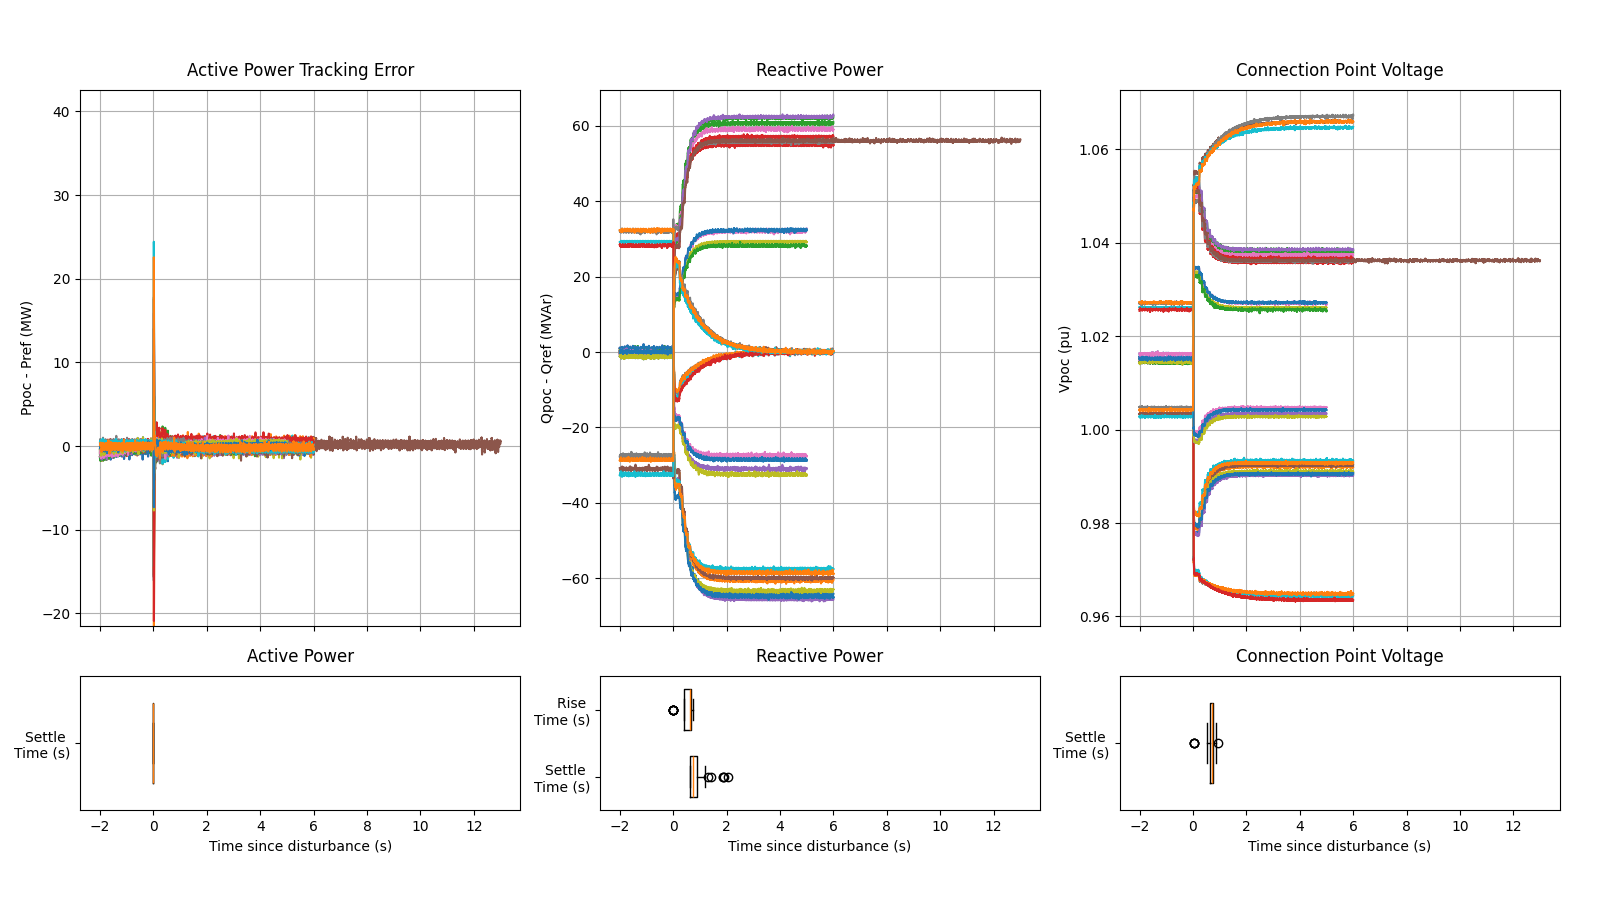
\includegraphics[width=0.9\textwidth]{\analysisdir/pscad/Vgrid step disturbance tracking.png}
		\caption{s5.2.5.13 Connection point voltage disturbance step test performance summary}
		\label{fig:s52513-vgrid-droop-step-summary-plot}
	\end{figure}
	
	Figure \ref{fig:s52513-vdroop-controller-accuracy} presents a summary of all $Q_{\mathrm{POC}}$ measurements against $V_{\mathrm{POC}}$ measurements at the end of each connection point voltage disturbance tests after the controllers have settled. It can be seen from this chart that the controller always accurately regulates to the intended voltage droop characteristic. Step changes have been applied that will cause the BESS to saturate into a reactive power limiter, which have been labelled as (sat) in the below test tables. These results are shown in full in Appendix \ref{Voltage Reference Step Tests}.
	
	\begin{figure}[H]
		\centering
		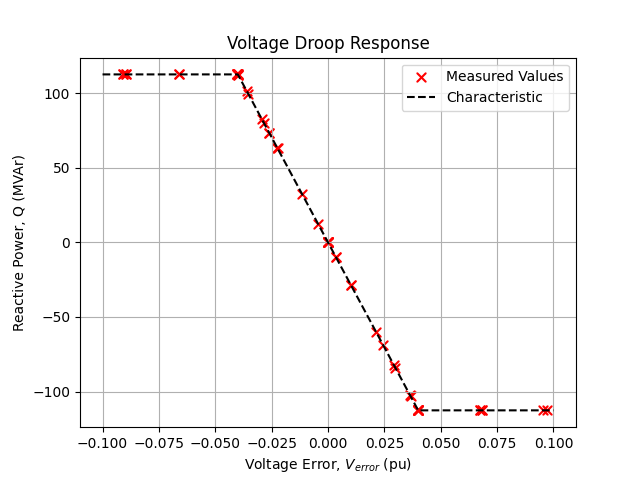
\includegraphics[width=0.7\textwidth]{\analysisdir/pscad/vdroop_characteristic.png}
		\caption{Voltage droop controller characteristic accuracy}
		\label{fig:s52513-vdroop-controller-accuracy}
	\end{figure}
	
	{
		\fontsize{9}{13}\selectfont
		\autoscaledlongtable
		{s5.2.5.13 Connection point voltage disturbance step test suite (droop mode)}
		{tab:s52513-vgrid-droop-step-table}
		{\projectassetsdir/test-suite-tables/52513-Vgrid-droop-test-table.csv}
	}
	

	\subsubsection{Voltage reference step tests}
	
	The connection point voltage reference step tests performed for this clause have been presented in Table \ref{tab:s52513-vref-step-table}. Figure \ref{fig:s52513-vref-step-summary-plot} show the tracking error (reference minus measurement) for reactive power and voltage, along with the distribution of rise and settling times (as applicable). The results show compliance to the GPS requirements for all tests. Active power recovery has not been tracked for these reference step changes, as no significant change in active power (>10\% of plant rating) was observed for these tests, and therefore calculating recovery was not practicable.
	
	
	\begin{figure}[H]
		\centering
		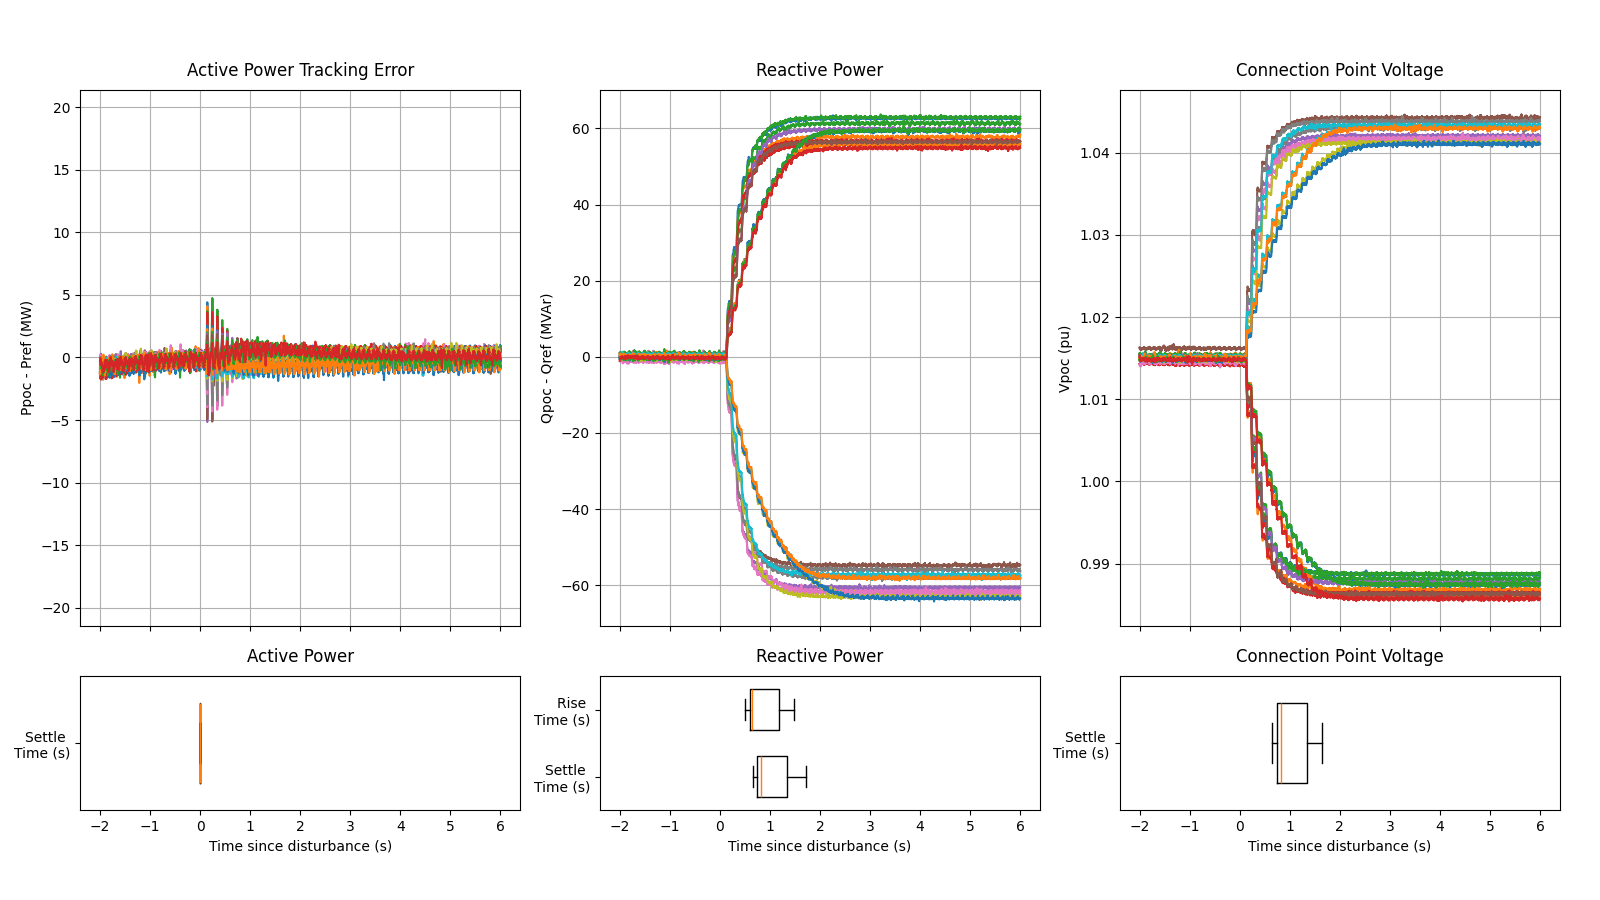
\includegraphics[width=0.9\textwidth]{\analysisdir/pscad/Vref step disturbance tracking.png}
		\caption{s5.2.5.13 Voltage reference step test performance summary}
		\label{fig:s52513-vref-step-summary-plot}
	\end{figure}

	
	{
		\fontsize{9}{10}\selectfont
		\autoscaledlongtable
		{s5.2.5.13 Voltage reference step test suite}
		{tab:s52513-vref-step-table}
		{\projectassetsdir/test-suite-tables/52513-Vref-test-table.csv}
	}
	
	Table \ref{tab:s52513-vref-step-results-table} shows the rise and settling times for each test performed.
	
	{
		\fontsize{9}{10}\selectfont
		\autoscaledlongtable
		{s5.2.5.13 Voltage reference step test results}
		{tab:s52513-vref-step-results-table}
		{report-assets/analysis/pscad/Vref step disturbance tracking.csv}
	}
	
	\subsubsection{Reactive power reference step tests}
	
	The connection point reactive power reference step tests performed for this clause have been presented in Table \ref{tab:s52513-qref-step-table}. Figures \ref{fig:s52513-qref-step-summary-plot} show the tracking error (reference minus measurement) for reactive power and voltage, along with the distribution of rise and settling times (as applicable). The results show compliance to the GPS requirements for all tests. Active power has not been tracked for these reference step changes, as no large change in active power (>10\% of plant rating) was observed for these tests, and therefore calculating recovery was not practicable. Full results for these tests are shown in Appendix \ref{Reactive Power Reference Step Tests}.
	
	
	\begin{figure}[H]
		\centering
		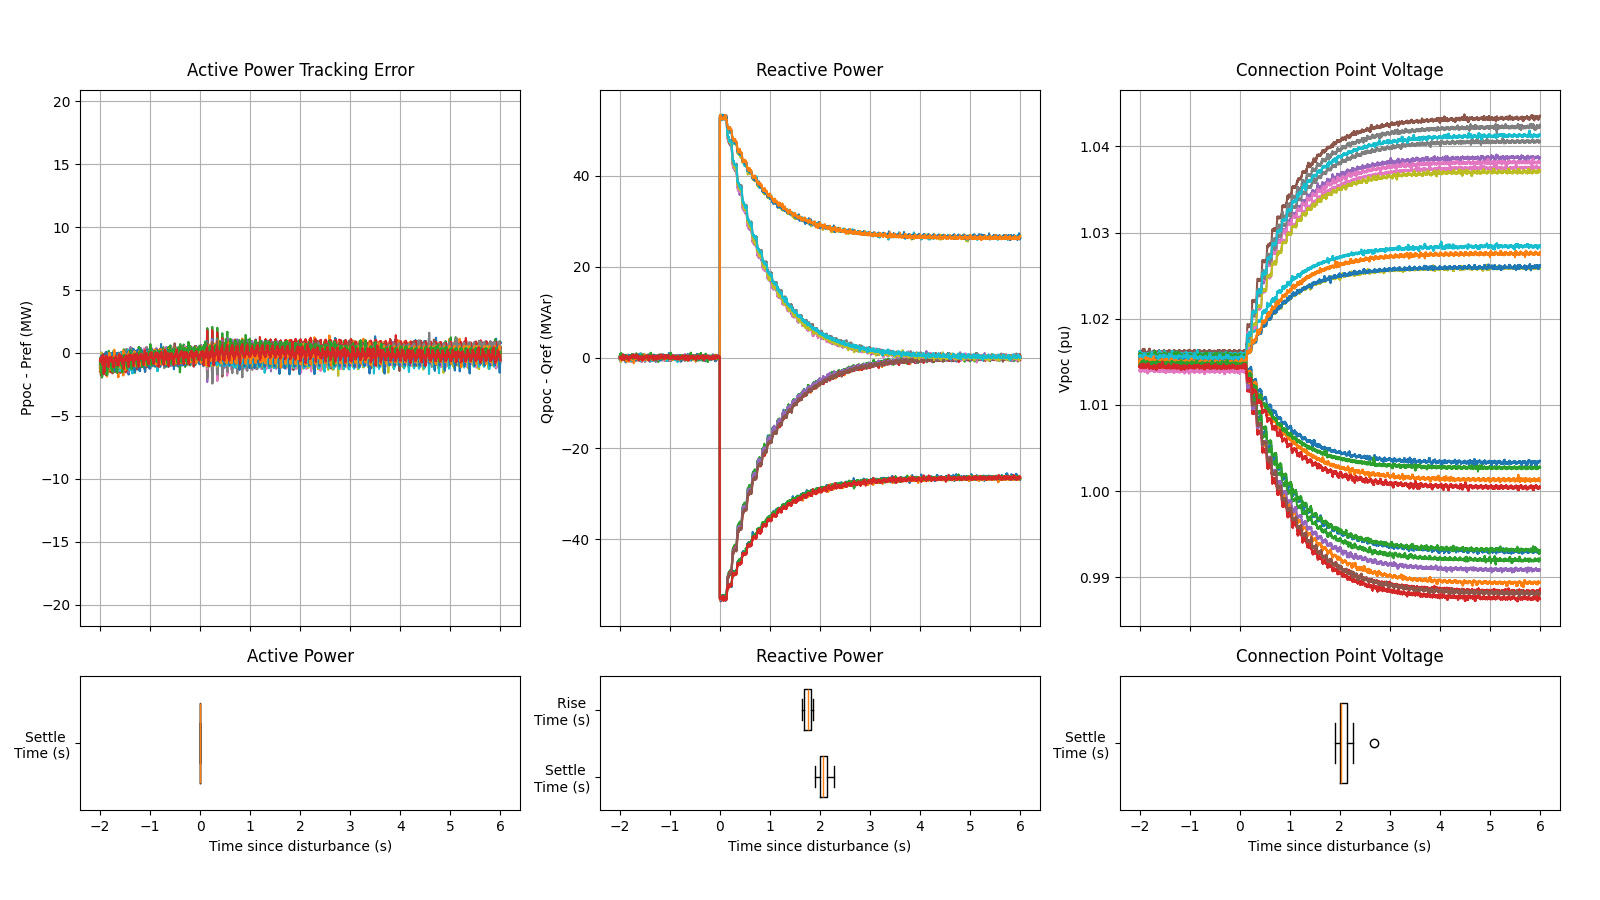
\includegraphics[width=0.9\textwidth]{\analysisdir/pscad/Qref step disturbance tracking.png}
		\caption{s5.2.5.13 VAr reference step test performance summary (saturating)}
		\label{fig:s52513-qref-step-summary-plot}
	\end{figure}
	
	{
		\autoscaledlongtable
		{s5.2.5.13 VAr reference step test suite}
		{tab:s52513-qref-step-table}
		{\projectassetsdir/test-suite-tables/52513-Qref-test-table.csv}
	}
	
	Table \ref{tab:s52513-qref-step-results-table} shows the rise and settling times for each test performed.
	
	{
		\fontsize{9}{10}\selectfont
		\autoscaledlongtable
		{s5.2.5.13 VAr reference step test results}
		{tab:s52513-qref-step-results-table}
		{report-assets/analysis/pscad/Qref step disturbance tracking.csv}
	}
	
	\subsubsection{Power factor reference step tests}
	
	The connection point power factor power reference step tests performed for this clause have been presented in Table \ref{tab:s52513-pfref-step-table} \ref{fig:s52513-pfref-step-unsaturated-summary-plot} show the tracking error (reference minus measurement) for reactive power and voltage, along with the distribution of rise and settling times (as applicable). The results show compliance to the GPS requirements for all tests. Active power has not been tracked for these reference step changes, as no large change in active power (>10\% of plant rating) was observed for these tests, and therefore calculating recovery was not practicable. Full results for these tests are shown in Appendix \ref{Power Factor Reference Step Tests}.
	
	
	\begin{figure}[H]
		\centering
		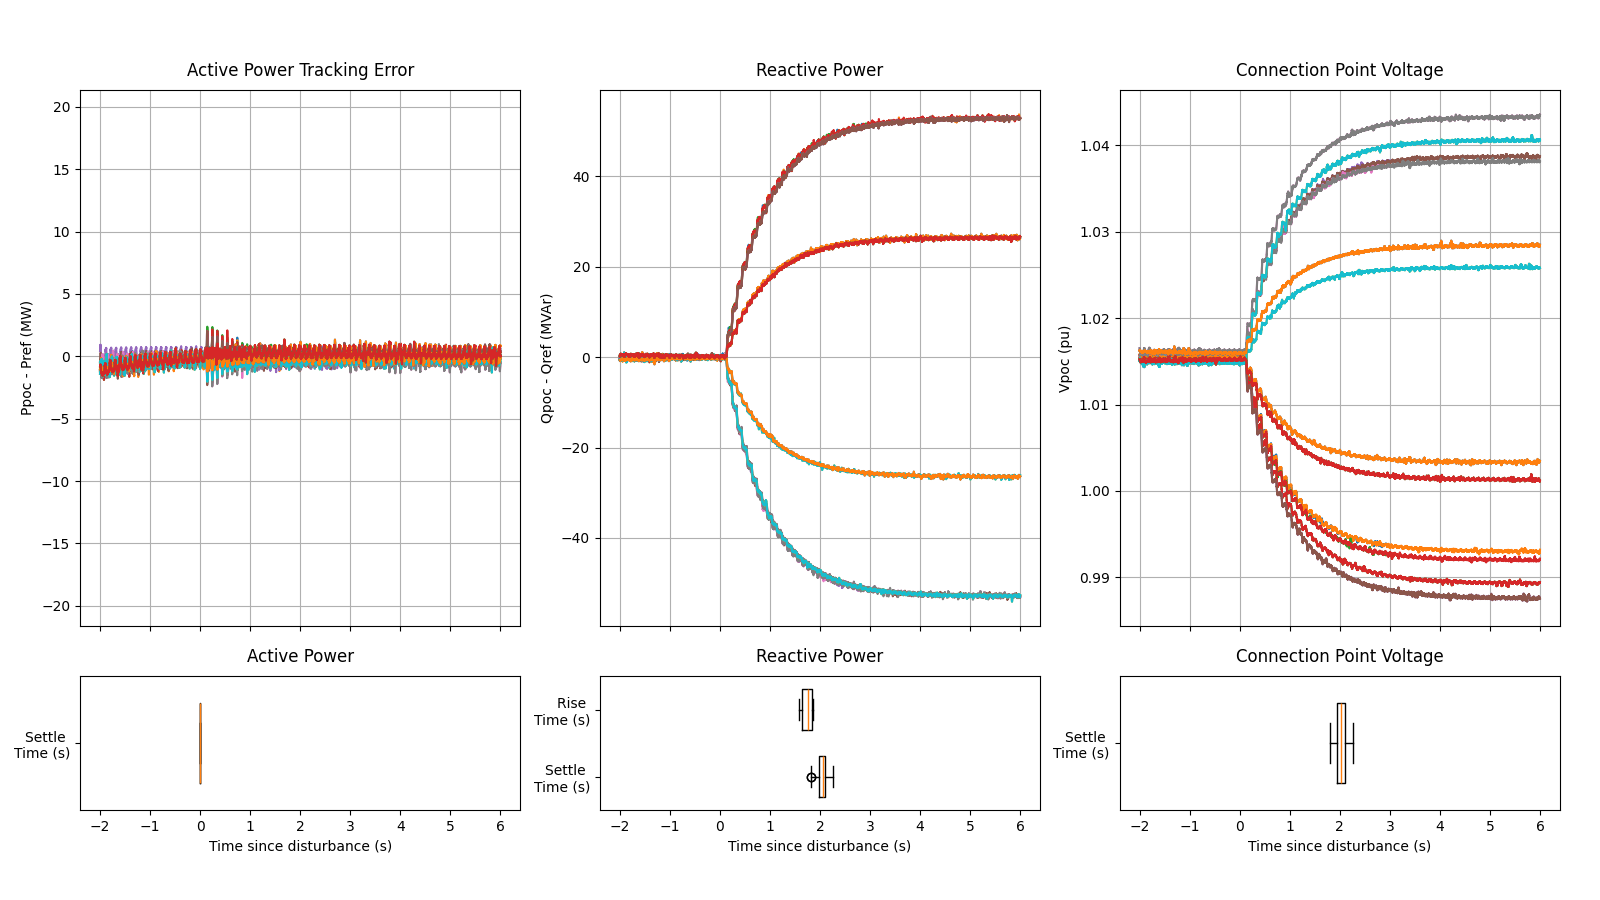
\includegraphics[width=0.9\textwidth]{\analysisdir/pscad/PFref step disturbance tracking.png}
		\caption{s5.2.5.13 PF reference step test performance summary (not saturating)}
		\label{fig:s52513-pfref-step-unsaturated-summary-plot}
	\end{figure}
	
	{
		\fontsize{9}{10}\selectfont
		\autoscaledlongtable
		{s5.2.5.13 PF reference step test suite}
		{tab:s52513-pfref-step-table}
		{\projectassetsdir/test-suite-tables/52513-PFref-test-table.csv}
	}
	
	Table \ref{tab:s52513-pfref-step-results-table} shows the rise and settling times for each test performed.
	
	{
		\fontsize{9}{13}\selectfont
		\autoscaledlongtable
		{s5.2.5.13 PF reference step test results}
		{tab:s52513-pfref-step-results-table}
		{report-assets/analysis/pscad/PFref step disturbance tracking.csv}
	}
	
	\subsection{Wide area study results}
	
	\subsubsection{Voltage reference step tests}
	
	The connection point voltage reference step tests performed in the wide area PSSE network have been presented in Table \ref{tab:s52513-wan-vref-step-table}. The results show compliance to the GPS requirements for all tests.
	
	Note that the accuracy of the controller has already been established in Section \ref{subsec:s52513-vgrid-steps-droop-mode} and assessment is therefore not repeated in \ac{WAN} studies.

	
	{
		\fontsize{9}{10}\selectfont
		\autoscaledlongtable
		{s5.2.5.13 \ac{WAN} voltage reference step test suite}
		{tab:s52513-wan-vref-step-table}
		{\projectassetsdir/test-suite-tables/wan-52513-Vref-test-table.csv}
	}
	
	Table \ref{tab:s52513-wan-vref-step-results-table} shows the rise and settling times for each test performed.
	
	{
		\fontsize{9}{10}\selectfont
		\autoscaledlongtable
		{s5.2.5.13 \ac{WAN} voltage reference step test results}
		{tab:s52513-wan-vref-step-results-table}
		{report-assets/analysis/psse-wan/Vref step disturbance tracking-wan.csv}
	}


	\section{[S5.2.5.14] Active Power Control}
	\subsection{Proposed Access Standard}
	\textbf{Automatic Access Standard}
		\begin{tcolorbox}[lightgreenbox]
			The integrated resource system has an active power control system that is adequately damped and capable of:
\begin{enumerate}
	\item maintaining and changing its active power level in accordance with its dispatch instructions; 
	\item ramping its active power level linearly from one dispatch level to another; and
	\item receiving and automatically responding to signals delivered from the automatic generation control system, as updated at a rate of once every 4 s  
\end{enumerate}

		\end{tcolorbox}
	\subsection{Assessment Methodology}
	
	Active power reference step tests assess the ability of the generator to provide a damped active (and reactive) power response to a change in the active power target applied to the PPC.

To perform this test, the generator is first initialised to the initial $V_{\mathrm{POC}}$, $P_{\mathrm{POC}}$, $Q_{\mathrm{POC}}$, SCR and X/R conditions, where $P_{\mathrm{POC}} = P_{\mathrm{ref}_{\mathrm{1}}}$. Once the generator has been initialised, the series of active power references $P_{\mathrm{ref}_{\mathrm{2}}}, P_{\mathrm{ref}_{\mathrm{3}}} \dots, P_{\mathrm{ref}_{\mathrm{n}}}$ are applied to the PPC, as shown in Figure~\ref{fig:smib-pref-change-methodology}.

\begin{figure}[h]
	\centering
	\newcommand{\bushere}[3]{% length, text above, text below}
% Optional arguments do nto work in paths
%
% starting point; draw an edge and then two nodes
% save the position
coordinate(tmp)
% go up and do an edge down
++(0,#1) node[anchor=base, font=\footnotesize]{#2} edge[ultra thick] ++(0, {-2*#1})
% edges do not move the current point, go down to position the node
++(0,{-2*#1}) node[below]{#3}
% go back to where we started
(tmp)
}

\ctikzset{sources/fill=gray!20, resistors/fill=gray!20}
\resizebox{\linewidth}{!}{ % Set width to \linewidth
	\begin{tikzpicture}[semithick]% default line width
		% Buses and branches
		\draw (0,0)
		node[left, font=\footnotesize]{Generator} ++(1.5,0) \bushere{1.5}{Connection Point}{} coordinate(poc);
		\draw (poc)
		-- ++ (1,0) to[generic, l={$Z_{\text{grid}}$}, resistors/width=2] ++ (4,0)
		-- ++ (1,0)
		\bushere{1.5}{Infinite Bus}{} coordinate(infinite bus);
		% One load (start from the coord load, go up)
		\ctikzset{bipoles/border margin=0.5}% See manual section 3.1.2
		\draw (infinite bus) -- ++(1,0) node[vsourcesinshape, rotate=90]{} coordinate(vgrid) ++(0.5,0) node[right]{$V_{\text{grid}}$};
		\draw (poc) -- ++(-1,0) node[vsourcesinshape, rotate=90]{} coordinate(generator);
		% Fault
		\draw[blue, font=\footnotesize, <-] (generator) ++(0, -0.5) -- ++(0, -0.5) -- ++(-0.5,0) node[left]{$P_{\mathrm{ref}_{\mathrm{1}}}, P_{\mathrm{ref}_{\mathrm{2}}}, P_{\mathrm{ref}_{\mathrm{3}}}, \dots, P_{\mathrm{ref}_{\mathrm{n}}}$};
		
	\end{tikzpicture}
}






	\caption{Active power reference change methodology}
	\label{fig:smib-pref-change-methodology}
\end{figure}
	
	All assessments for this clause have been performed in PSCAD.

	\subsection{Results}
	
	The full set of active power control tests are shown in Tables \ref{tab:s52514-test-suite} and \ref{tab:s52514-test-suite-CRG}, which were ran as part of the DMAT testing. The results demonstrate that the generating system is capable of ramping stably without a defined ramp rate limit. The ramp rate of the generator is also configurable, allowing the generator to set a required ramp rate to reach a target on the next 5 minute interval, which will be dynamically selected by the SCADA system.)\footnote{The specific ramp rate for a given scenario will be calculated by the upstream controllers, which are not modelled in PSCAD or PSS/E.}. These results can be viewed in the DMAT Appendix G.
		
	\begin{table}[H]
		\centering
		\caption{s5.2.5.14 active power control test suite}
		\label{tab:s52514-test-suite}
		\autoscaledtable{H}{\projectassetsdir/test-suite-tables/3211-Pref-test-table.csv}
	\end{table}
	
	\begin{table}[H]
		\centering
		\caption{s5.2.5.14 active power control test suite - charging}
		\label{tab:s52514-test-suite-CRG}
		\autoscaledtable{H}{\projectassetsdir/test-suite-tables/3211-Pref-CRG-test-table.csv}
	\end{table}
	
	\section{[S5.2.5.15] Short Circuit Ratio}
	\subsection{Proposed Access Standard}
	\textbf{Negotiated Access Standard - SCR of 1.2}
		\begin{tcolorbox}[lightgreenbox]
		The integrated resource system comprised of asynchronous generating units must have plant capability sufficient to operate stably and remain connected at a short circuit ratio (SCR) of 1.2, assessed in accordance with the methodology prescribed in the system strength impact assessment guidelines, where:
\begin{enumerate}
	\item the rated active power for calculating the SCR value is 285MW.
\end{enumerate}

	\end{tcolorbox}
	\subsection{Assessment Methodology}
	The ability of the plant to comply with this proposed standard and operate at a short circuit ratio of 1.2 is assessed by a full System Strength impact assessment undertaken by the Network Service Provider. As part of this connection application per advice from AEMO, studies have been carried out using the \ac{LMTH} PSCAD model to assess the ability of the grid-forming technology to operate at an SCR of 1.2. The short circuit ratio of the project can fall to 1.06 during a single contingency of the 220 kV line between Ballarat and Learmonth, however due to static stability limitations in a SMIB environment, the floor for assessment is currently set at 1.2. Sungrow do not currently certify their PSSE model as being capable of representing the plant response at SCR levels below 1.5, and therefore assessment of capability has been conducted using the PSCAD model for the plant only. This assessment has included:
	\begin{itemize}
		\item SCR change faults - where grid impedance is modified to an SCR of 1.2 following a fault on the network.
		\item Frequency changes at SCR 1.2 - small frequency step changes were applied to the network to test the ability of the plant to remain stably connected under small step changes (0.5 Hz at 4 Hz/s).
		\item Small voltage (5\%) step changes at SCR 1.2.
	\end{itemize}
	
	Full results for operation at 1.2 can be seen in the PSCAD DMAT appendices O-Q.

	\subsection{Results}
	For all the small disturbances modelled, inclusive of frequency and voltage disturbances, the plant was capable of remaining in continuous uninterrupted operation. No significant issues were observed with operation at low SCR for these studies in the SMIB model. An example of small voltage disturbances applied at the point of connection at SCR 1.2 is shown in Figure \ref{fig:52515-voltage-steps}.
	
	\begin{figure}[H]
		\centering
		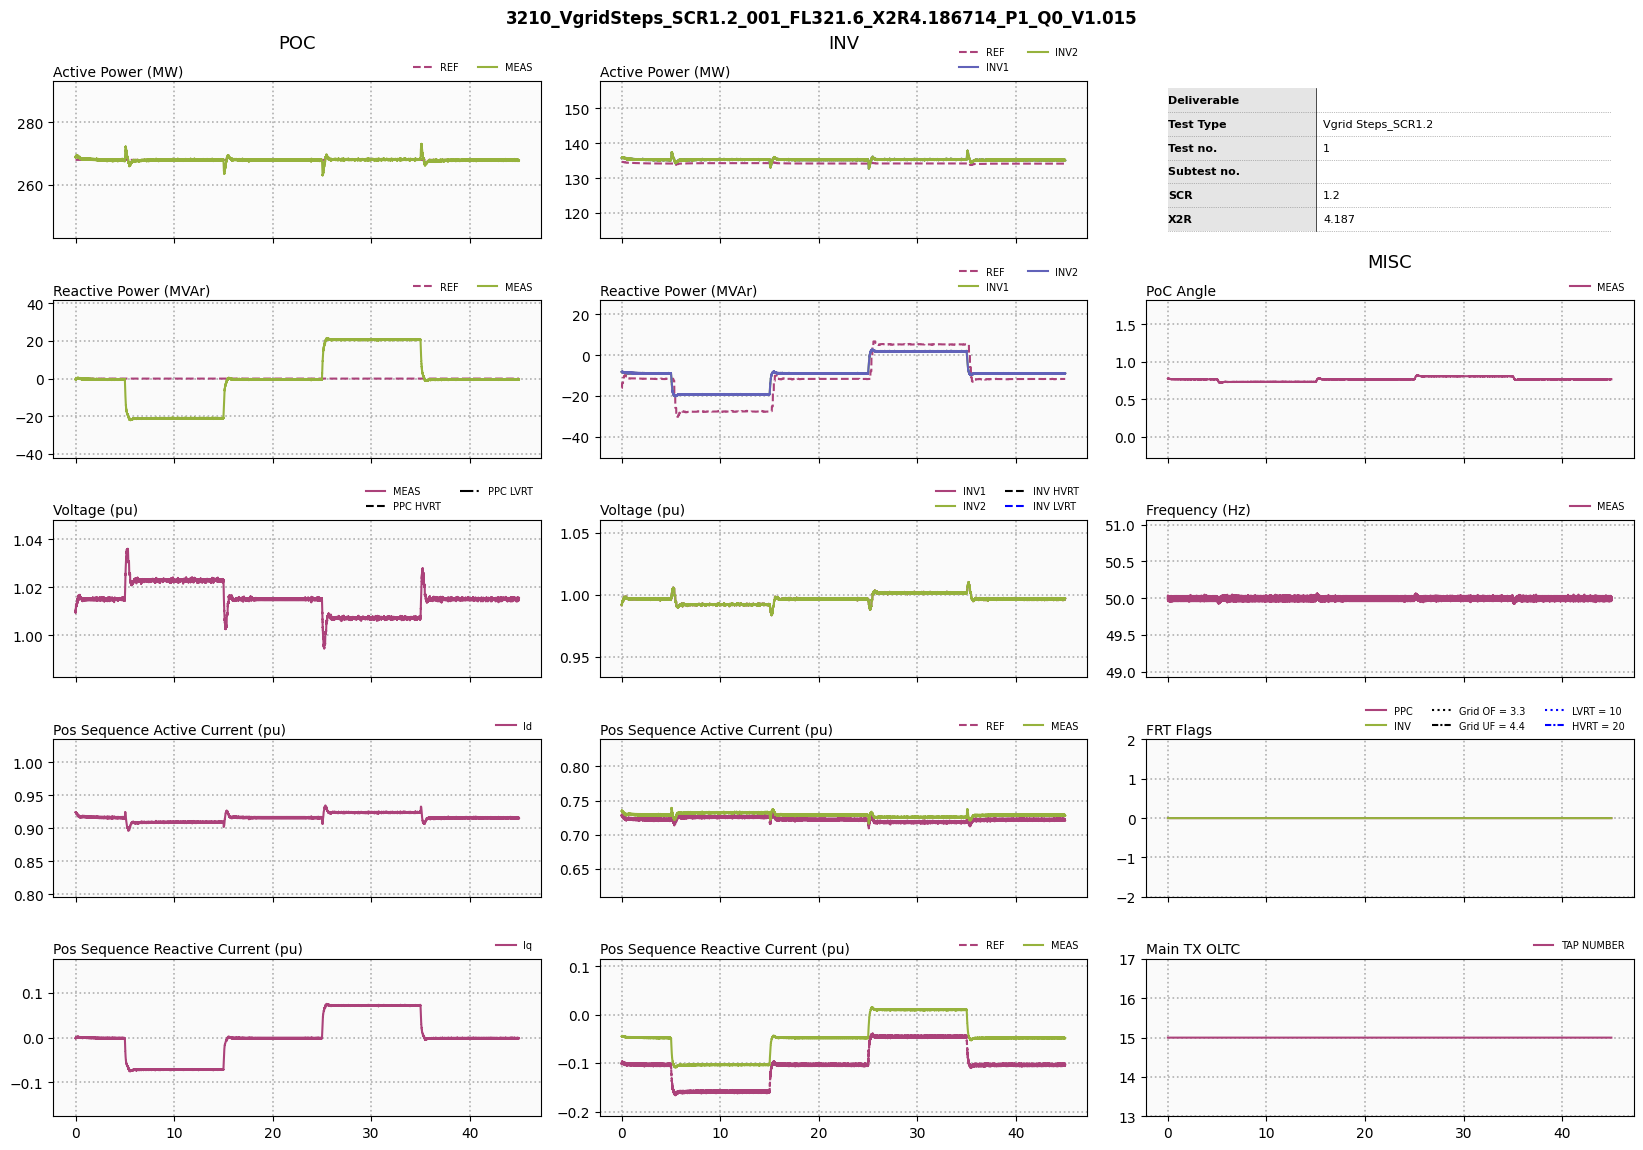
\includegraphics[width=0.7\textwidth]{\analysisdir/pscad/3210_VgridSteps_SCR1.2_001_FL321.6_X2R4.186714_P1_Q0_V1.015.png}
		\caption{s5.2.5.15 voltage step changes at SCR 1.2 (PSCAD)}
		\label{fig:52515-voltage-steps}
	\end{figure}
	
	An example of the small frequency disturbances applied is shown in Figure \ref{fig:52515-frequency-steps}, showing the BESS remains stable even when its inertial response causes it to exceed its rated active power. 
	
	\textbf{It should be noted that large frequency disturbances which cause the plant to respond and exceed the transient stability limit will cause the SMIB model to collapse at SCR 1.2.} The inertial and droop frequency response of the plant has been tuned in order to avoid this condition for small frequency disturbances (0.5 Hz disturbances at up to 4 Hz / s), however this will not apply for increasingly large frequency step changes at a high RoCoF. This is an issue in a SMIB testing environment where the static power transfer limit applies. If this is considered to be a risk to stability likely to be present outside of a testing environment, alternative options for resolution of this issue can be considered.
	
	\begin{figure}[H]
		\centering
		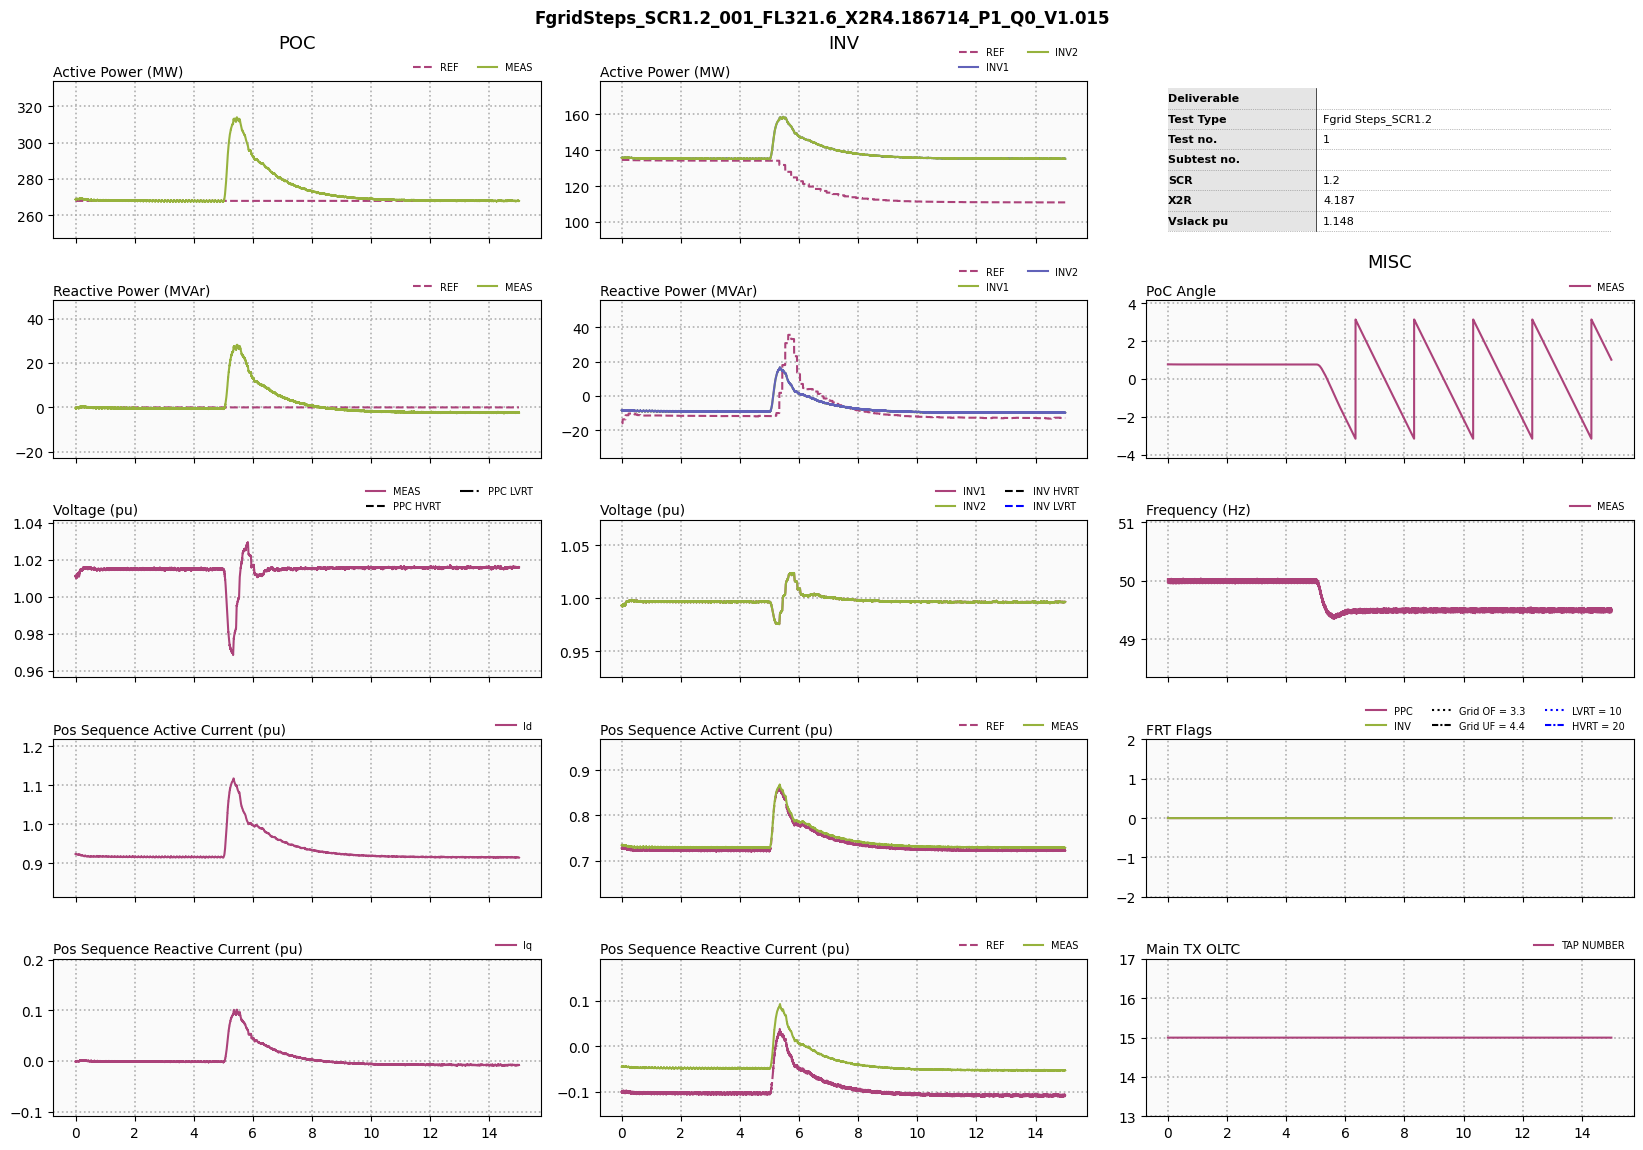
\includegraphics[width=0.7\textwidth]{\analysisdir/pscad/FgridSteps_SCR1.2_001_FL321.6_X2R4.186714_P1_Q0_V1.015.png}
		\caption{s5.2.5.15 frequency step changes at SCR 1.2 (PSCAD)}
		\label{fig:52515-frequency-steps}
	\end{figure}
	
	For the large disturbances tested, where SCR change was carried out in conjunction with a fault, issues were observed with the SMIB environment that required additional testing. These issues were set out in a technical note to AEMO. \cite{scr-change-tech-memo} The \ac{IRP} was not capable of operating following an SCR change when charging at minimum rated power, due to the BESS breaking the static stability limit for a SMIB model under these conditions. AEMO provided feedback on alternative testing methodology to be carried out, specified in their System Strength methodology review document \cite{system-strength-methodology-review}, which specified acceptable slack voltages to carry out testing at in order to determine an acceptable stability limit for the BESS while discharging.
	
	In line with AEMO's methodology, additional tests were carried out at 1.2 SCR and at expected system X to R ratio under these conditions, to validate that the control systems of the BESS were able to remain in continuous uninterrupted operation when the static stability limit was not breached. A full list of tests undertaken is presented in Table \ref{tab:static-stability-tests}, with a full set of results visible in Appendix \ref{Static Limit Testing}.
	
		\begin{table}[H]
		\centering
		\caption{Static stability limit tests - charging at SCR 1.2}
		\label{tab:static-stability-tests}
		\autoscaledtable{H}{\projectassetsdir/test-suite-tables/SCR-Change-Faults-Testing-test-table.csv}
		\end{table}
		
	The testing found that the plant remained connected and stable following a reduction in active power when charging, dispatched up to 70\% of rated minimum active power at multiple reactive power setpoints.
	
	No limitations were noted when the BESS was discharging, with the plant capable of operating up to its rated active power of 268 MW when dispatched at an SCR of 1.2. A standard of 1.2 is therefore proposed for this clause, pending completion of a system strength final impact assessment.
	
	
	\section{[S5.2.5.8] Fault Current}
	\subsection{Proposed Access Standard}
	\textbf{Automatic Access Standard}
	\begin{tcolorbox}[lightgreenbox]
		\begin{itemize}
	\item The generating system limits its contribution to the fault current at the Connection Point to:
	\begin{itemize}
		\item Three-phase fault current: 1.57 kA;
		\item Single-phase-to-ground fault current: 4.7 kA;
		\item Phase-to-phase-to-ground fault current: 2.71 kA.
	\end{itemize}
	\item The generating system’s connected plant is capable of withstanding fault current through the connection point up to 40 kA for 1000 ms.
	\item The circuit breaker provided to isolate the generating system from the network is capable of breaking, without damage or restrike, the maximum fault current of 40 kA, expected to flow through the circuit breaker for any fault in the network or in the generating system.
\end{itemize}

	\end{tcolorbox}
	\subsection{Assessment Methodology}
	
	This assessment was undertaken using the PowerFactory model of the plant, using data provided by Sungrow to calculate converter maximum fault contribution.\cite{sungrow-fault-level} The IEC60909 method was used for fault level analysis, which takes a c-factor of 1.1 at the 220 kV point of connection. Ik'' values at 100 ms were used to populate this standard.
	
	The \ac{GPS} has been set based on a 10\% tolerance to the study result. This is to account for any reticulation or transformer impedance changes which may occur as a result of manufacturing tolerances or detailed design change requirements. 
	
	The withstand rating of the plant is subject to detailed design, but will be rated consistently with the requirements of AEMO's guidelines for connection in Victoria, which requires equipment is rated to withstand an ultimate fault current of 40 kA when connecting at 220 kV.
	
	\subsection{Results}
	
	The fault contribution at the point of connection from the plant was:
	\begin{itemize}
		\item Three phase fault current - 1.423 kA
		\item Single-phase-to-ground fault current - 4.263 kA
		\item Phase-to-phase-to-ground fault current - 2.461 kA
	\end{itemize}

	
	% The Heywood Battery Energy Storage System (HEYWOODBESS) is a $\pm~285MW/1140MWh$ Battery Energy Storage Project, is located 5 km from the town of Heywood and 300 km west of Melbourne in Victoria as shown in Figure~\ref{fig:project-location}. The project is expected to connect directly to the existing 275 kV Heywood terminal station via a single high voltage cable.

HEYWOODBESS will include 92 SMA Sunny Central 4.6 MVA (SCS 4600 UP-S) converters which will be connected to two 275/33/33kV, 160MVA three winding transformers through a 33kV reticulation system. Each converter will have a dedicated 33/0.69kV, 4.6 MVA step up transformer.


\begin{figure}[H]
	\centering
	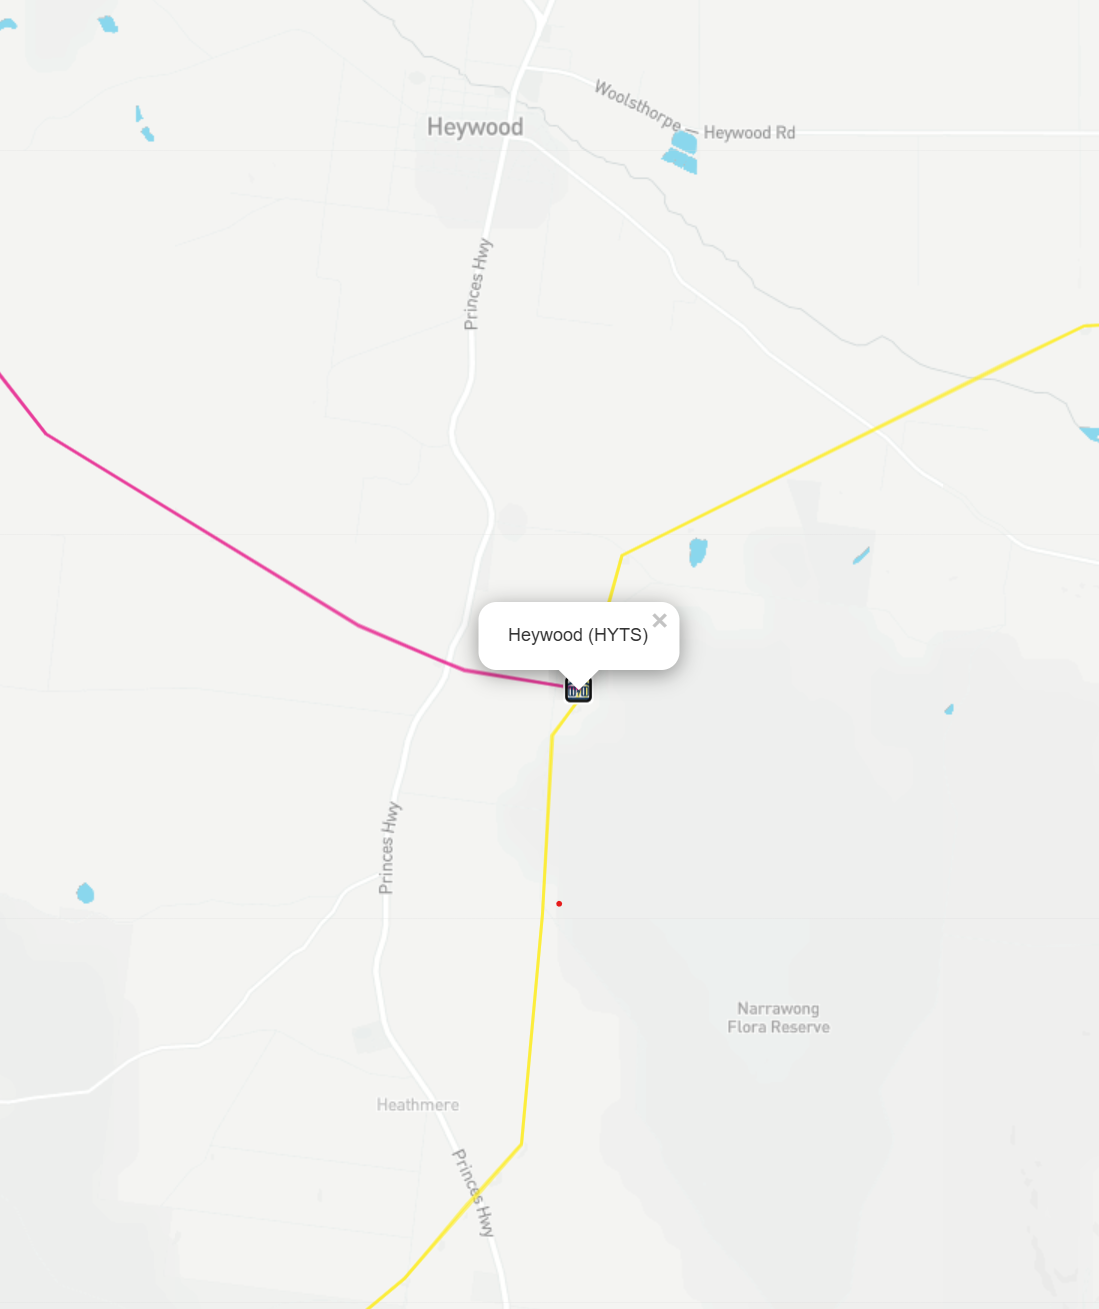
\includegraphics[width=0.7\textwidth]{\projectassetsdir/project-location.png} % Change example-image-a to the filename of your image
	\caption{Project location}
	\label{fig:project-location}
\end{figure}


	
	\chapter*{Acronyms}
\begin{acronym}%[JSONP]\itemsep0pt
	\acro{AAS}{Automatic Access Standard}
	\acro{AEMO}{Australian Energy Market Operator}
	\acro{VSL}{Voltage Stackable Logic}
	\acro{AGC}{Automatic Generation Control}
	\acro{AVR}{Automatic Voltage Regulator}
	\acro{BESS}{Battery Energy Storage System}
	\acro{BOP}{Balance Of Plant}
	\acro{CGBESS}{Clements Gap BESS}
	\acro{Heywood BESS}{Heywood Battery Energy Storage System}	
	\acro{CSR}{Connection Studies Report}
	\acro{CT}{Current Transformer}
	\acro{CUO}{Continuous Uninterrupted Operation}
	\acro{HV}{High Voltage}
	\acro{DMAT}{Dynamic Model Acceptance Test}
	\acro{DYR}{PSSE Dynamics Data File}
	\acro{EMT}{Electromagnetic Transients}
	\acro{FIA}{Full Impact Assessment}
	\acro{FRT}{Fault Ride-Through}
	\acro{GPS}{Generator Performance Standards}
	\acro{HVRT}{High Voltage Ride-Through}
	\acro{LV}{Low Voltage}
	\acro{LVRT}{Low Voltage Ride-Through}
	\acro{MV}{Medium Voltage}
	\acro{NEM}{National Electricity Market}
	\acro{NSP}{Network Service Provider}
	\acro{OEM}{Original Equipment Manufacturer}
	\acro{OFRT}{Over-Frequency Ride-Through}
	\acro{OLTC}{On-Load Tap Changer}
	\acro{OPDMS}{Operations and Planning Data Management System}
	\acro{OVRT}{Over-Voltage Ride-Through}
	\acro{PLL}{Phase-Locked Loop}
	\acro{PLR}{Partial Load Rejection}
	\acro{PPC}{Power Plant Controller}
	\acro{PPM}{Power Plant Manager}
	\acro{RoCoF}{Rate of Change of Frequency}
	\acro{RMS}{Root Mean Square}
	\acro{RMU}{Ring Main Unit}
	\acro{RUG}{Releasable User Guide}
	\acro{S5251}{Reactive Power Capability}
	\acro{S5254}{Generating System Response to Voltage Disturbances}
	\acro{SCR}{Short Circuit Ratio}
	\acro{SMIB}{Single Machine, Infinite Bus}
	\acro{SLD}{Single Line Diagram}
	\acro{TOV}{Temporary Over-Voltage}
	\acro{UFRT}{Under-Frequency Ride-Through}
	\acro{UVRT}{Under-Voltage Ride-Through}
	\acro{VCS}{Voltage Control Strategy}
	\acro{WAN}{Wide Area Network}
	\acro{WF}{Wind Farm}
	\acro{VOIP}{Voice Over Internet Protocol}
	\acro{VRR}{Voltage Regulation Relay}
	\acro{VT}{Voltage Transformer}
\end{acronym}
	\renewcommand\bibname{References}

\begin{thebibliography}{99}	
	\bibitem{mvps-sld}MVPS SLD\\
	(PSD1834-110-001-002.pdf)
	\bibitem{mvt-datasheet}Medium Voltage Transformer Datasheet\\
	(CG_D_00181175_03_General MVT Datasheet.pdf.pdf)
	\bibitem{main-tx-datasheet} Main Transformer Datasheet\\
	(Main Transformer Datasheet.pdf)
	\bibitem{substation-sld} Substation SLD\\
	(PSD1834-110-001-001.pdf)
	\bibitem{avr-manual}TAPCON 230 AVR manual\\
	(bal_3552133_02_001_1_en.pdf)
	\bibitem{oltc-switching} OLTC Switching Datasheet\\
	(VACUTAP®_VV®_Operating_Instructions.pdf)
	\bibitem{harmonic-assessment} Harmonic Emmissions Report\\
	(PSD1834-100-100---Harmonic-Emissions-Assessment-and-Filter-Design-Rev-B.pdf)
	\bibitem{scada-philo} SCADA Control Philosophy\\
	(PSD1834-200-009---SCADA-CONTROL-PHILOSOPHY-Rev.3.pdf)
	\bibitem{aemo-io} AEMO IO Schedule\\
	(PSD1834-200-005-AEMO IO SCHEDULE-REV-04.pdf)
	\bibitem{comms-arch} Communication Architecture\\
	(PSD1834-210-003-001---COMMUNICATION-ARCHITECTURE-Rev.1.pdf)
	\bibitem{scada-spec} SCADA Functional Specification\\
	(PSD1834-200-001 - SCADA SYSTEM FUNCTIONAL DESIGN SPECIFICATION Rev.4.pdf)
	\bibitem{protection-settings-report} Protection Settings Report\\
	(PSD1834-100-007---CGBESS-Protection-Setting-Report---REV-C.pdf)



\end{thebibliography}

	
	\newpage
	\appendix
	\renewcommand{\thesection}{\Alph{section}}  % Change section numbering to A, B, C, etc.
	\setcounter{section}{0}  % Start the section counter at 0 (which will be labeled "A")
	
	\section*{Appendices}
	\addcontentsline{toc}{section}{Appendices}  % Add to the Table of Contents
	
	\section{Reactive Power Capability Curve Data}
	\label{Reactive Power Capability Curve Data}
	
	\section{Grid Frequency Disturbance Withstand Tests}
	\label{Grid Frequency Disturbance Withstand Tests}
	
	\section{Grid Voltage Disturbance Withstand Tests}
	\label{Grid Voltage Disturbance Withstand Tests}
	
	\section{Grid Frequency Disturbance Step Tests}
	\label{Grid Frequency Disturbance Step Tests}
	
	\section{Grid Voltage Disturbance Step Tests}
	\label{Grid Voltage Disturbance Step Tests}
	
	\section{Power Factor Reference Step Tests}
	\label{Power Factor Reference Step Tests}
	
	\section{Voltage Reference Step Tests}
	\label{Voltage Reference Step Tests}
	
	\section{Reactive Power Reference Step Tests}
	\label{Reactive Power Reference Step Tests}

	\section{Partial Load Rejection Tests}
	\label{Partial Load Rejection Tests}
	
	\section{Temporary Over-Voltage Tests}
	\label{Temporary Over-Voltage Tests}
	
	\section{Continuous Uninterrupted Operation}
	\label{Continuous Uninterrupted Operation}
	
	\section{Static Limit Testing}
	\label{Static Limit Testing}
	
	\section{Autumn High - Wide Area Network Contingency Results}
	\label{Autumn High - Wide Area Network Contingency Results}

	\section{Autumn Low Export - Wide Area Network Contingency Results}
	\label{Autumn Low Export - Wide Area Network Contingency Results}
	
	\section{Autumn Low Import - Wide Area Network Contingency Results}
	\label{Autumn Low Import - Wide Area Network Contingency Results}
	
	\section{Wide Area Network Steady State Results}
	\label{Wide Area Network Steady State Results}

	

	
\end{document}